% Overleaf-ready skeleton generated from MANUSCRIPT_v2.md. Text is a STARTING POINT: rewrite in your own words, add \cite{} keys (see refs.bib), delete the red [VERIFY] tags once checked.
% Journal templates: Elsevier journals (CMIG, CBM) -> elsarticle.cls (documentclass[review]{elsarticle}); Springer (JIIM) -> sn-jnl.cls. Switch the class and keep the \input lines.
\documentclass[11pt,a4paper]{article}
\usepackage[utf8]{inputenc}\usepackage[T1]{fontenc}\usepackage{lmodern}
\usepackage[margin=2.2cm]{geometry}\usepackage{graphicx,booktabs,xcolor,hyperref,amsmath,caption,subcaption,float,natbib}
\hypersetup{colorlinks=true,linkcolor=blue!50!black,citecolor=blue!50!black,urlcolor=blue!50!black}
\graphicspath{{figures/}}
\title{How reliable are radiograph body-part classifiers? A leakage-controlled, cross-dataset benchmark with reliability and label-quality analysis on public data}
\author{Sheikh Noor Abdullah$^{1,*}$\thanks{Corresponding author. ORCID: \href{https://orcid.org/0009-0002-7193-4284}{0009-0002-7193-4284}} \and A.B.M. Kabir Hossain$^{1}$\\[4pt]
{\small $^{1}$Department of Information and Communication Engineering, Bangladesh Army University of Engineering \& Technology (BAUET),\\ Qadirabad Cantonment, Natore, Bangladesh}\\[2pt]
{\small $^{*}$Corresponding author: \texttt{sheikhnoorabdullah02@gmail.com}; \texttt{kabir111192@gmail.com}}}
\date{}
\begin{document}\maketitle
\begin{abstract}\textbf{Background.} Published accuracies for radiograph body-part classification are hard to compare: splits, thresholds and uncertainty are rarely reported, and most large studies use private data.
\textbf{Methods.} We built a leakage-controlled benchmark on the public UNIFESP dataset (22 classes, 1,738 radiographs, 768 patients) with patient-level folds, a 323-image held-out set, all choices made on out-of-fold predictions and patient-bootstrap confidence intervals. We added ablations, a frozen foundation-model baseline, transfer to MURA and FracAtlas, a MURA benchmark, calibration and selective prediction, and a label audit.
\textbf{Results.} The ensemble reached a held-out sample-mean F1 of 0.919 (95 \% CI 0.867 to 0.960), not significantly above its best single model (+0.0066, p = 0.063); no ablation differed from the reference (all p > 0.08). A gated CNN-Transformer fusion ignored its CNN branch. A random image-level split overstated validation F1 by 0.0144 (patient-level folds: 0.0004), and tuning thresholds on the scored set added 0.0083. On the official MURA validation set accuracy was 0.9747 (0.9663 to 0.9818), against 0.9643 reported by Shah et al. for the same images. The ensemble was well calibrated (ECE 0.054), and accuracy on retained images rose from 0.926 to 0.945 at 90 \% coverage. The audit flagged 39 of 1,415 training images (2.8 \%) as possible label errors, unreviewed by clinicians. A late Kaggle submission without pseudo-labels scored 0.9256 (private), between second and third place.
\textbf{Conclusion.} How a classifier is evaluated matters more than its architecture: gains from fusion, ensembling and pseudo-labelling fell within the noise of a 323-image held-out set.


\end{abstract}
\noindent\textbf{Keywords:} body-part classification; radiograph; data leakage; reproducibility; calibration; label noise
\section{Introduction}
A radiograph usually reaches the archive with its anatomical region stored in a DICOM tag or a free-text study description, and either can be wrong or missing. An early audit of 562 images found false \emph{Body Part Examined} entries in 15.3 \% of them (Güld et al., SPIE 2002). Deep networks can read the region from the pixels instead (Pham et al. 2021; Langer et al. 2024; Mitsuyama et al. 2025). Most of that work uses private data, reports accuracy alone and says little about how the splits and thresholds were chosen.
On the public UNIFESP dataset (Farina, Abdala and Kitamura) we found one academic paper, which reports 86.94 \% accuracy for the best of five CNNs (Krishnan and Padmavathi 2025). That study treated the 1,738 training images as a single-label 22-class problem, added 1,088 GAN-generated images to the 1,686 originals, and reports accuracy only; we could not find a description of a patient-level split or of a held-out protocol, and a Kaggle competition whose final private leaderboard is led by a score of 0.93378. Two evaluation shortcuts are known to inflate results in other fields: leakage between images of the same patient, and thresholds or checkpoints chosen on data that is later scored (Kapoor and Narayanan 2023; Roberts et al. 2021). We did not find a measurement of how large these effects are for body-part classification A search of PubMed, arXiv and general web sources in November 2026 found studies of leakage in other imaging tasks but none that measured it for radiograph body-part classification..
So instead of chasing the leaderboard we asked two questions. How much of the reported performance survives a leakage-controlled protocol? And what would a clinical router need besides accuracy? The paper contributes:
\begin{itemize}\item a reproducible, patient-level benchmark on public data with confidence intervals (Tables 1 and 2);\item a measurement of how much common shortcuts inflate scores (Tables 4 and 5);\item negative results: no ablation, fusion variant or ensembling step was significantly better, and a gated CNN-Transformer fusion collapsed onto one branch (Tables 4 and 6);\item results on MURA and FracAtlas, including a body-part benchmark on the official MURA split (Tables 7 to 9);\item calibration, risk-coverage and a label audit based on out-of-fold predictions, aimed at routing use (Section 5.7);\item a frozen foundation-model baseline with a label-efficiency curve (Section 5.6) and a Grad-CAM faithfulness check (Table 10).\end{itemize}


\section{Related work}
\textbf{Body-part classification.} Pham et al. (2021) sorted 16,093 images into five coarse groups for DICOM routing (recall 0.982) and pointed out that routing needs near-perfect accuracy. Langer et al. (2024, preprint) classified 14 regions on 48,434 hospital radiographs (96.6 \% for a single model, 97.7 \% for an ensemble). When experts reviewed the test errors, 35 \% turned out to be wrong labels and 11 \% were out-of-domain images, so label noise accounts for part of the remaining error.

Mitsuyama et al. (2026) trained a seven-category model (Head, Neck, Chest, Incomplete Chest, Abdomen, Pelvis, Extremities) on 429,341 radiographs from two institutions and MURA, and tested it on a second institution and on MURA. Every MURA image was labelled "Extremities", and micro-accuracy on MURA was 98.6 \% (99 \% CI 98.4 to 98.7 \%). Radiologist review changed the DICOM-derived body-part label of 3.9 \% of the radiographs from one institution and 12.8 \% from the other. Their MURA figure cannot be compared with ours: theirs is a coarse seven-way task in which all MURA images share one class, whereas we separate the seven MURA study types.

On MURA, Shah et al. (2026) classified the seven upper-extremity study types with an attention-fused Xception-Swin model and reached an accuracy of 0.9643, a macro-F1 of 0.9574 and an AUC of 0.9963. They used the public validation set (3,197 images) as the test partition, a fixed seed (42), a patient-wise data organisation and image-level evaluation, and they report Wilson confidence intervals for the abnormality-detection accuracies; we did not find intervals or repeated seeds for the body-part result. All of these studies differ from ours in data, class set and metric.

\textbf{Hybrid CNN-Transformer models} with gated or attention-based fusion are common. We did not find a report that inspects the learned gate, although absence from our search does not prove absence from the literature. \textbf{Hierarchical losses} have also been tried: Wu, Tygert and LeCun (2019) found that minimising a hierarchical loss directly is difficult, and that minimising cross-entropy often lowers it almost as well, which makes it more useful as a metric than as a training objective.

\textbf{Evaluation quality.} Leakage is widespread in machine-learning-based science (Kapoor and Narayanan, 2023) and in COVID-19 imaging (Roberts et al., 2021). Label quality limits medical-imaging benchmarks (Oakden-Rayner, 2020), and reporting guidance exists in the CLAIM 2024 update (Tejani et al., 2024). Oakden-Rayner (2020) audited MURA labels and found them more accurate than those of ChestX-ray14, although the normal/abnormal labels were unreliable for cases with degenerative joint disease. Confident-learning methods find label errors from out-of-fold probabilities (Northcutt et al., 2021).



\section{Data}
\textbf{UNIFESP} (Farina, Abdala and Kitamura, Kaggle; CC BY-NC-SA 4.0) holds 2,481 DICOM radiographs. They are de-identified, come from the Universidade Federal de São Paulo under IRB approval, and the Kaggle version is reduced to 256 $\times$ 256 pixels. Radiology residents labelled them on the MD.ai platform, with 20 body regions plus "Others", in a multilabel scheme. The dataset page names four residents; it does not say how many readers saw each image, whether disagreements were adjudicated, or who the patients were. There are 1,738 training images from 768 patients (63 \% of patients have several images) and 743 test images from 330 patients whose labels are hidden. No patient appears in both sets. Ninety-five percent of the images are MONOCHROME1 (inverted). The DICOM \emph{BodyPartExamined} tag is empty in all 2,481 files, so we could not measure the tag error rate on this dataset. Of the training images, 92.4 \% carry one label (122 carry two, 10 carry three), and class frequency runs from 738 (Chest) down to 9 (Clavicles). A random forest on metadata alone (photometric interpretation, bits stored, size; patient-grouped cross-validation) reached accuracy 0.486 against 0.451 for the majority class, with macro-F1 0.059, so acquisition metadata hold almost no label information.
\textbf{Splits.} We split by patient with multilabel stratification (iterative stratification, seed 42). That gave a fixed held-out set of 323 images from 156 patients and a cross-validation pool of 1,415 images from 612 patients in five folds. The held-out set has only 1 to 3 positives for Clavicles (1), Skull (2), Forearm (3), Elbow (3) and Thigh (3), so per-class numbers for these classes are unstable.
\textbf{Other datasets.} For \textbf{MURA} (Rajpurkar et al. 2018) we took the body part from the \texttt{XR\_*} folder name (7 classes) and used the official train/validation split. \textbf{FracAtlas} (Abedeen et al., Sci Data 2023, CC BY 4.0) has 4,083 images from three hospitals in Bangladesh, annotated by two radiologists and an orthopaedist; we used the 3,685 with a single region (hand, hip, leg or shoulder) for zero-shot transfer. \textbf{COVID-19 Radiography} (Chowdhury et al. 2020) has 4 classes and no patient identifiers, so its split is image-level.

\textbf{Dataset availability.} All four datasets are public, but access conditions differ.
\begin{itemize}\item UNIFESP X-Ray Body Part Classification: \url{https://www.kaggle.com/datasets/felipekitamura/unifesp-xray-bodypart-classification} (doi:10.34740/KAGGLE/DSV/3399135; CC BY-NC-SA 4.0).\item MURA (v1.0): Stanford AIMI, \url{https://stanford.redivis.com/datasets/cv1a-apytk3j44} (project page \url{https://stanfordmlgroup.github.io/competitions/mura/}). Access requires AIMI membership and acceptance of the Stanford University School of Medicine Dataset Research Use Agreement (non-commercial, research-only use; redistribution of the data is not permitted). The first author holds approved access under this agreement (status checked on 6 November 2026). Because redistribution is prohibited we do not release MURA images or derived image files, only code, split lists and result files. The experiments reported here used a third-party Kaggle copy of MURA v1.1 (\url{https://www.kaggle.com/datasets/cjinny/mura-v11}, no description, licence unspecified) obtained before the official access was granted \textbf{\textcolor{red}{[VERIFY: compare the md5 hashes of the Kaggle files with the md5\_hash column of the official Redivis table]}}; the official validation split served as our held-out set because the official test set is hidden.\item COVID-19 Radiography Database: \url{https://www.kaggle.com/datasets/tawsifurrahman/covid19-radiography-database} (files (c) original authors; cite Chowdhury et al. 2020 and Rahman et al.).\item FracAtlas: figshare, doi:10.6084/m9.figshare.22363012 (CC BY 4.0). We used the Kaggle copy \url{https://www.kaggle.com/datasets/orvile/fracatlas} with 4,083 images as in the Scientific Data paper; the current figshare version (v7) lists 4,073 images, so the two are not identical.\end{itemize}
No new patient data were collected. Our code, split files, seeds and result files are provided with the submission [repository link on acceptance].


\section{Methods}
\textbf{Pre-processing.} We applied the DICOM rescale slope and intercept, inverted MONOCHROME1 images, normalised each image to 8 bit by its own minimum and maximum, replicated it to three channels and resized it to 224 pixels (Swin-T) or 256 pixels (all others). ImageNet mean and standard deviation were used for scaling.
\textbf{Models.} All backbones were ImageNet-pretrained timm models (Swin-T, DenseNet121, EfficientNetV2-S, ConvNeXt-T, ResNet50, EfficientNet-B3), each with a 22-way sigmoid head and a 22-way softmax head. For the fusion ablation we combined DenseNet121 and Swin-T in five ways: a learned gate on raw features, the same gate with LayerNorm, a fixed 0.5/0.5 average, the CNN branch alone, and the Swin branch alone.
\textbf{Training.} We used AdamW (weight decay 1e-4; learning rate 2e-4 for Swin, 3e-4 for DenseNet, ResNet and EfficientNet, 1e-4 for ConvNeXt), a cosine schedule with one warm-up epoch, 30 epochs, batch size 32, fp16, an exponential moving average of the weights (0.998) and gradient clipping at 5. The loss was binary cross-entropy with positive weights capped at 20, plus 0.5 times a soft-target cross-entropy on the softmax head. Light augmentation was flip, shift-scale-rotate and brightness/contrast; heavy augmentation added noise and blur. We did not pick checkpoints: the final averaged weights were used.
\textbf{Decisions made on out-of-fold (OOF) predictions only.} These were the head and test-time-augmentation variant of each run, the ensemble weights (greedy Caruana selection, 40 iterations), the per-class thresholds (coordinate ascent on sample-mean F1, shrunk towards 0.5 with weight n\_pos/(n\_pos+20)) and the rule that every image gets at least one label. The held-out set was used once (Fig. 1).
\begin{figure}[htbp]\centering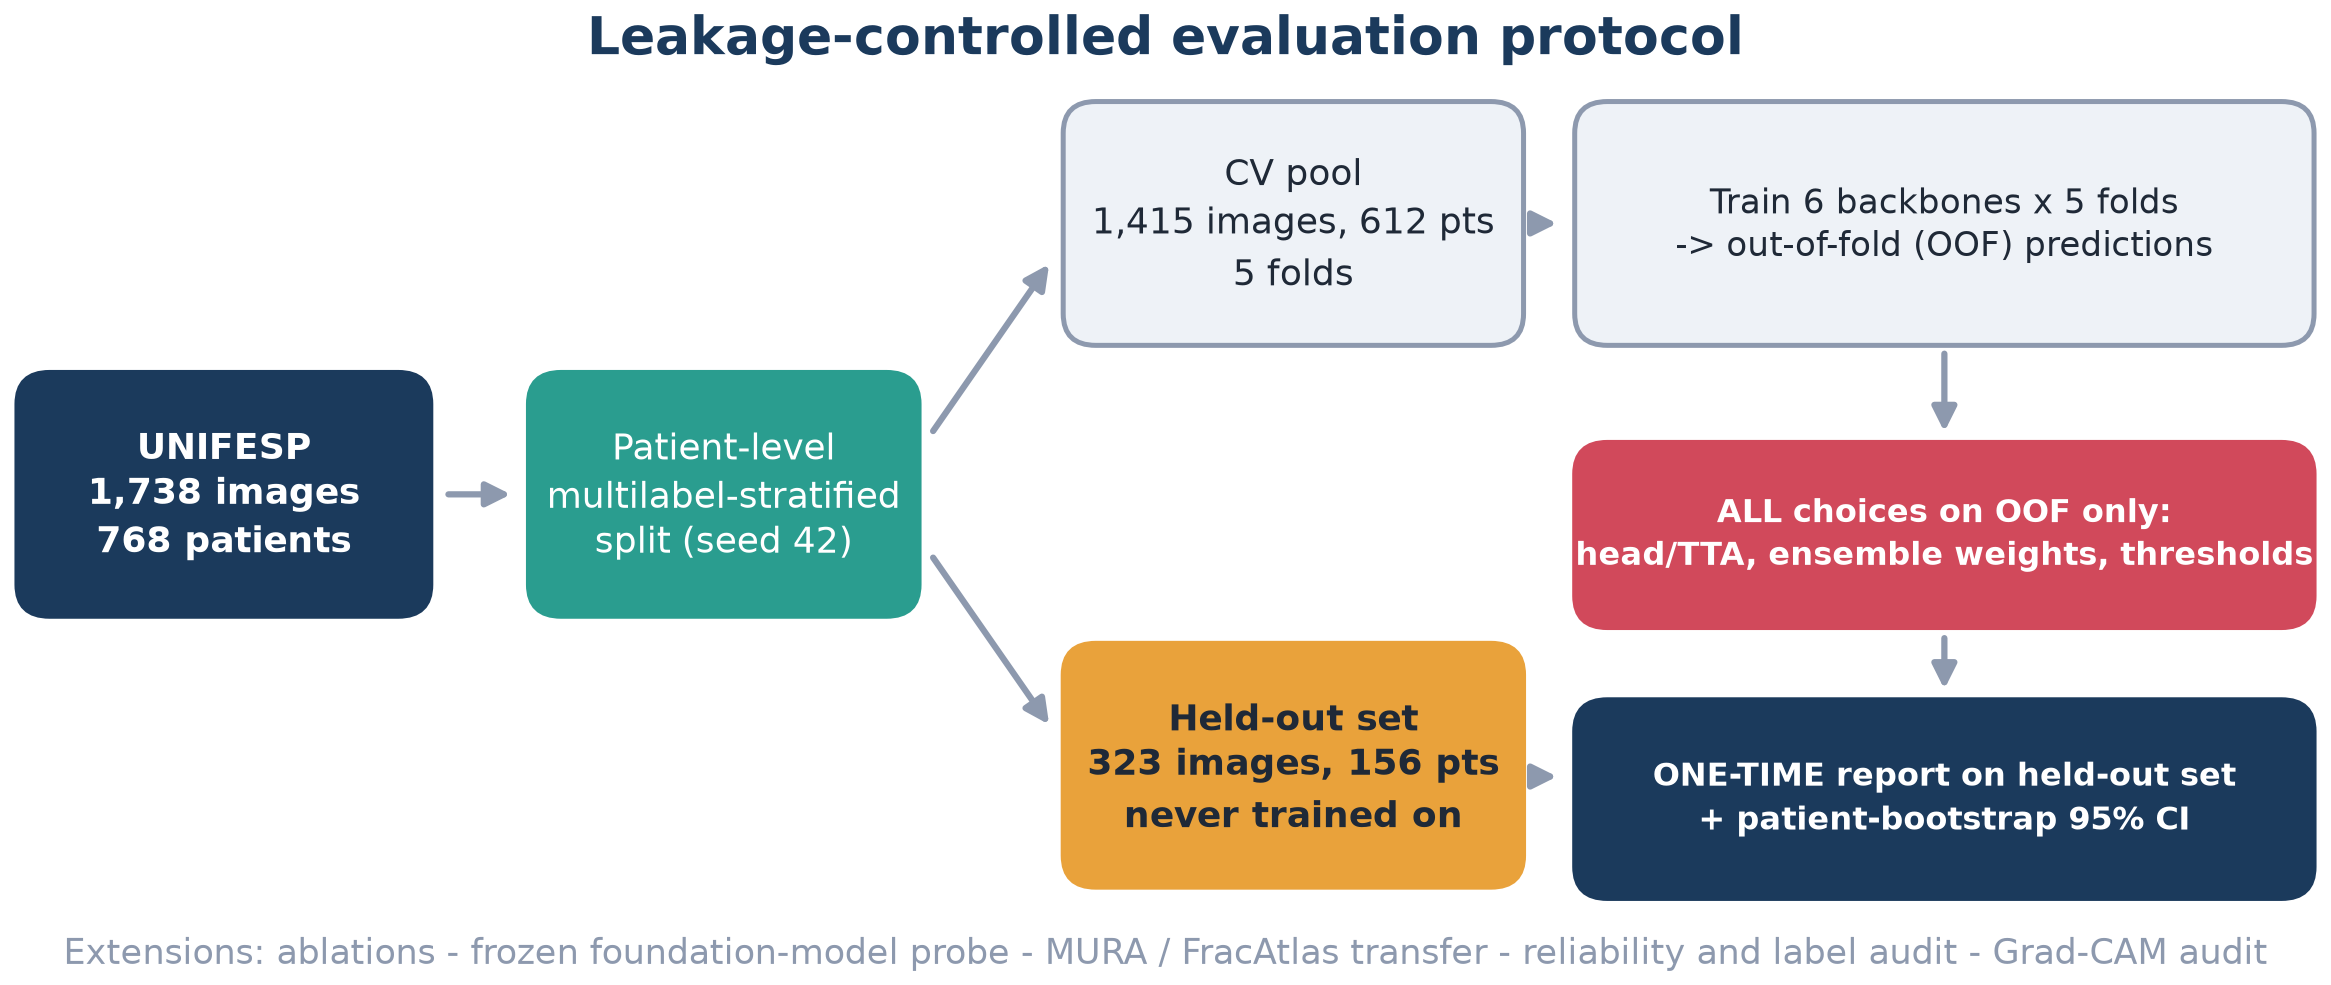
\includegraphics[width=0.95\textwidth]{fig1_protocol.png}\caption{Evaluation protocol. Images are split by patient into a cross-validation pool and a held-out set. Every choice is made on out-of-fold predictions, and the held-out set is scored once, with patient-bootstrap confidence intervals.}\label{fig:1}\end{figure}

\textbf{Metrics and statistics.} We report sample-mean F1 (the competition metric), macro-F1, micro-F1 and subset accuracy. Confidence intervals are 95 \% patient-level bootstrap intervals (2,000 resamples, or 1,000 for the reliability analysis), and model comparisons use a paired patient bootstrap. FracAtlas and the other transfer targets have no patient identifiers, so their intervals come from an image-level bootstrap and are optimistic.
\textbf{Frozen foundation-model baseline.} We froze DINOv2-S, DINOv2-B and an ImageNet Swin-T at 224 pixels, standardised the features on the cross-validation pool and trained a linear probe with 22 sigmoid outputs (binary cross-entropy plus L2). Weight decay was chosen on OOF predictions, and folds and held-out set were the same as before. To get a label-efficiency curve we repeated this with 10, 25, 50 and 100 \% of the training patients in each fold.
\textbf{Cross-dataset transfer.} We mapped the label spaces onto each other in a closed set (for example MURA hand, wrist and forearm onto the UNIFESP classes of the same name), restricted predictions to the shared groups and report accuracy and macro-F1. The map is our own assumption.
\textbf{Reliability analysis.} The ensemble combined five saved ablation runs (three Swin-T seeds, DenseNet121 and ConvNeXt-T) with weights fitted on OOF predictions. We measured top-1 calibration (ECE with 15 bins; temperature fitted on OOF, applied to the held-out set), drew a risk-coverage curve in which the model abstains on low-confidence images, and computed per-class precision, recall and F1 with patient bootstrap intervals. For the \textbf{label audit}, a training image counts as a \emph{suspect} when the OOF ensemble gives probability 0.9 or more to a class other than its given label and a low probability to the given one (as in confident learning). Suspects are not proven errors.
\textbf{Explainability.} We computed Grad-CAM maps for three fold-0 models on the held-out set, ran a deletion test against a random map on the same grid, and ran a randomisation sanity check.
\textbf{Hardware and software.} All runs used Kaggle notebooks on 2 $\times$ NVIDIA T4 GPUs (Stage 2 took 18,811 s) with PyTorch 2.11.0 (CUDA 13.0). The other libraries (timm, albumentations, pydicom, scikit-learn) were the versions preinstalled on the Kaggle image at the time of the runs, from October to November 2026; we did not record a full package list, which we list as a limitation. Code, split files and seeds are released on GitHub (Zenodo, doi:10.5281/zenodo.24027438).


\section{Results}
\subsection{Main result (UNIFESP held-out set; Table 2)}
The ensemble of six candidate runs (four received non-zero weight, see Table 2), with thresholds tuned on OOF predictions, reached a sample-mean F1 of 0.9189 [0.8669, 0.9602], macro-F1 0.8630 [0.6891, 0.8916], micro-F1 0.9148 and subset accuracy 0.8885. At a plain 0.5 threshold the first two values are 0.9164 and 0.8537. The best single run by OOF (ConvNeXt-T) reached 0.9123, so the ensemble gained +0.0066 [-0.0002, +0.0142] (p = 0.063). Single runs (Supplementary Table S1) lie between 0.910 and 0.922 (Fig. 6).

\setcounter{table}{0}
\Needspace*{9\baselineskip}
\begin{center}\begin{minipage}{\textwidth}\small
\captionof{table}{UNIFESP held-out performance (decisions made on out-of-fold predictions only)}\label{tab:main}
\resizebox{\textwidth}{!}{\begin{tabular}{lcccc}
\toprule
\textbf{decoding} & \textbf{sample-mean F1} & \textbf{macro-F1} & \textbf{micro-F1} & \textbf{subset acc.} \\
\midrule
ensemble, threshold 0.5 & 0.9164 & 0.8537 & 0.9130 & 0.8885 \\
ensemble, 0.5 + min-one & 0.9164 & 0.8537 & 0.9130 & 0.8885 \\
ensemble, per-class thresholds tuned on OOF + min-one & 0.9189 [0.8669, 0.9602] & 0.8630 [0.6891, 0.8916] & 0.9148 & 0.8885 \\
best single run by OOF (convnext\_tiny\_s256), 0.5 + min-one & 0.9123 & 0.8482 & 0.9070 & 0.8762 \\
\bottomrule
\end{tabular}}
\par\smallskip{\footnotesize Held-out set: 323 images / 156 patients; 95 \% CIs by patient-level bootstrap. Ensemble minus best single: +0.0066 [-0.0002, +0.0142], p = 0.063. Ensemble weights (OOF, Caruana): efficientnetv2\_s\_s256 0.10, convnext\_tiny\_s256 0.27, resnet50\_s256\_heavy 0.29, efficientnet\_b3\_s256\_hv 0.34.}
\end{minipage}\end{center}


\begin{figure}[t]\centering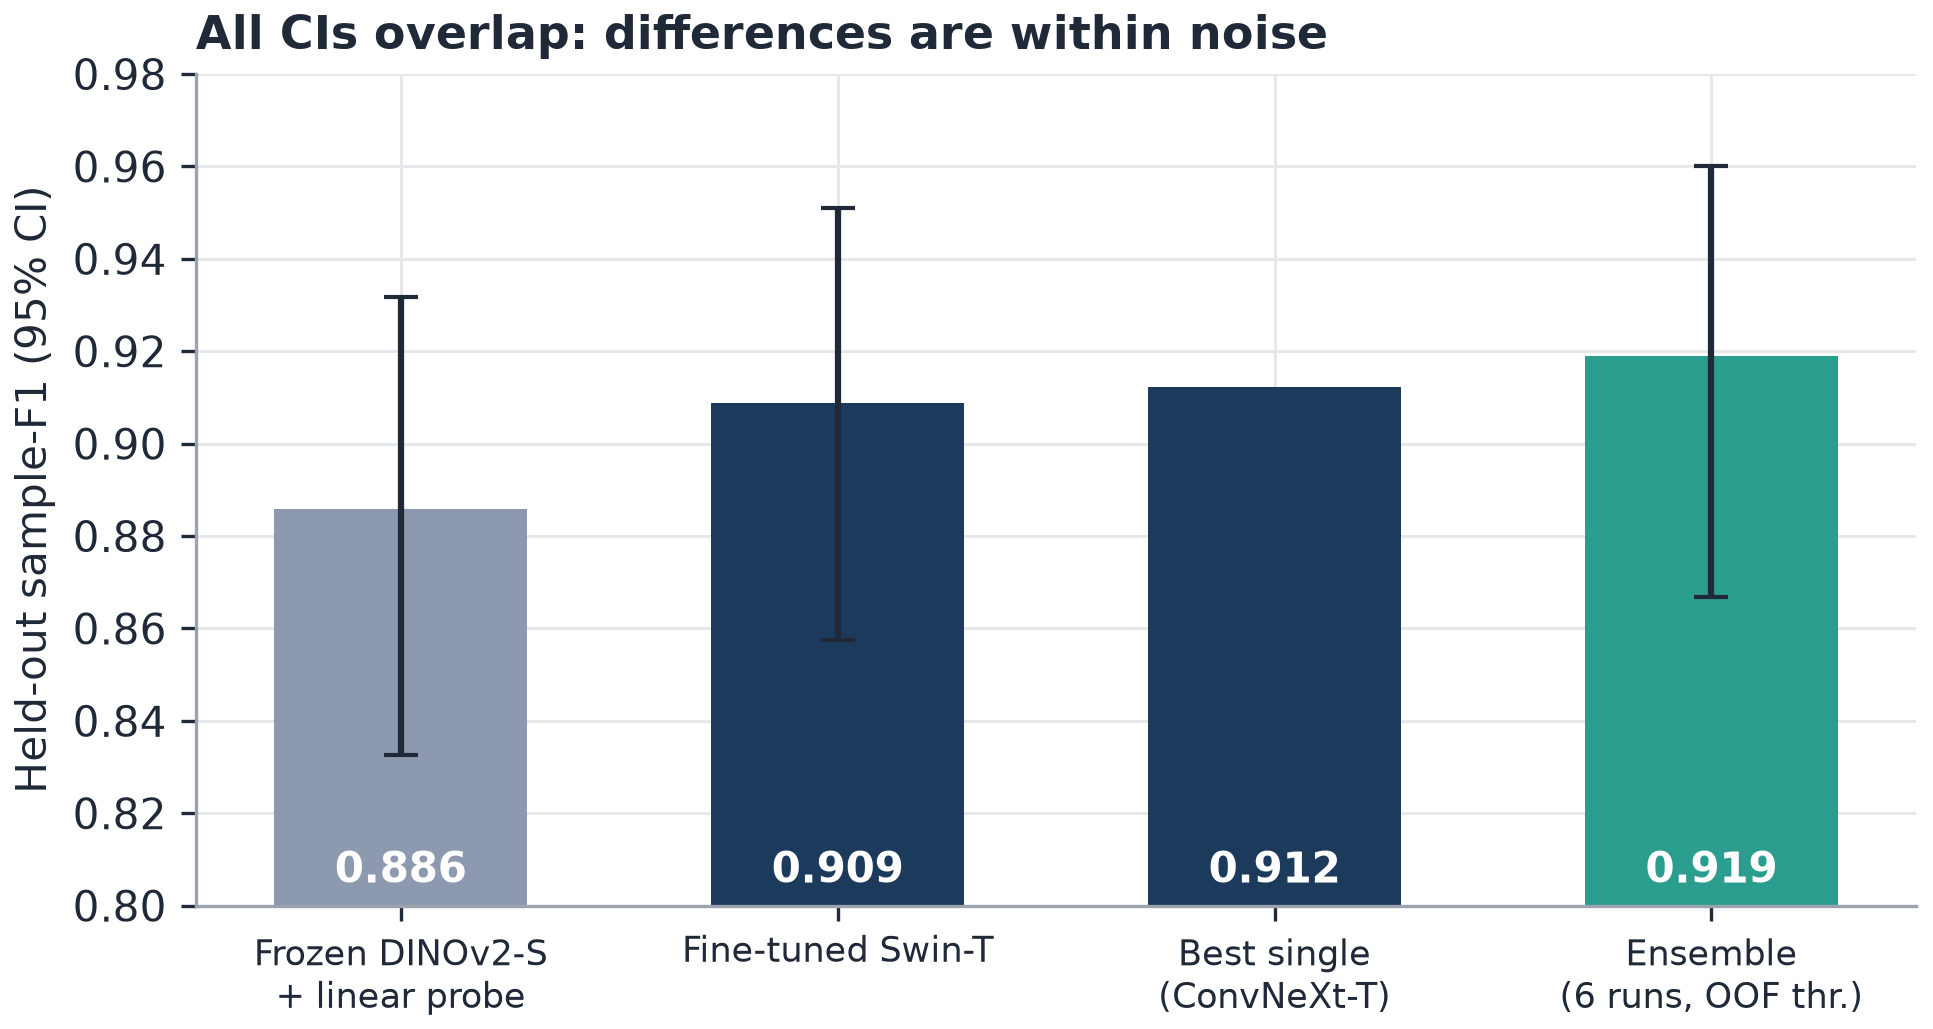
\includegraphics[width=0.8\textwidth]{fig10_heldout_overview.png}\caption{Held-out sample-F1 for a frozen DINOv2-S probe, the fine-tuned Swin-T, the best single model and the ensemble. All 95 \% confidence intervals overlap.}\label{fig:6}\end{figure}\suppressfloats[t]

\subsection{Competition score (Table 3)}
Both late submissions are unranked, and we report every submission we made. The Stage 1 ensemble scored 0.92563 on the private leaderboard and 0.92704 on the public one; the Stage 2 ensemble of 16 models scored 0.92638 and 0.93378. The final private leaderboard has 0.93378 in first place, 0.92787 in second and 0.92488 in third, so both of our submissions would sit between second and third place.

\begin{table}[t]
\centering\small
\caption{Kaggle UNIFESP private score vs. the competition leaderboard}\label{tab:kaggle}
\resizebox{\textwidth}{!}{\begin{tabular}{lcc}
\toprule
\textbf{entry} & \textbf{private\_score} & \textbf{public\_score} \\
\midrule
\#1 Harshit Sheoran & 0.93378 &  \\
\#2 JGK (ResNet50/152, FastAI) & 0.92787 &  \\
ours: stage-2 union (late submission) & 0.92638 & 0.93378 \\
ours: stage-1 ensemble (late submission) & 0.92563 & 0.92704 \\
\#3 Colin Greeley & 0.92488 &  \\
\#4 KobeU Systems Medicine & 0.92414 &  \\
\#5 wangkui & 0.92182 &  \\
\bottomrule
\end{tabular}}
\par\smallskip{\footnotesize Mean F1 (sample-wise); private score uses \textasciitilde{}60 \% of the test set with the original (partly noisy) labels, so differences of \textasciitilde{}0.003 are within noise. Late submissions are not listed on the leaderboard; report ALL submissions made.}
\end{table}


The private score uses about 60 \% of the 743 test images and their original, partly noisy labels. We estimate its standard error at about 0.012, which means the gap to first place (0.0074) cannot be resolved and the gain of Stage 2 over Stage 1 (+0.00075) is indistinguishable from noise.

Stage 2 was evaluated differently, with OOF predictions on all 1,738 training images, so its numbers are not comparable with the held-out results (Table 4). The plain ensemble of 8 models scored 0.9262 [0.9092, 0.9414]. The same models retrained with pseudo-labels from 539 of the 743 unlabelled test images (confidence 0.9 or higher) scored 0.9233 [0.9058, 0.9392], and the union of all 16 models scored 0.9279 [0.9116, 0.9428]. In paired patient-bootstrap comparisons the union beat the plain ensemble by +0.0017 [-0.0010, +0.0046] (p = 0.25), and the pseudo-labelled models fell short of it by 0.0029 [-0.0092, +0.0034] (p = 0.36). Pseudo-labelling on its own did not help. It lowered both OOF F1 and macro-F1 (the latter from 0.8749 to 0.8587). The union's small gain rests on weights fitted to the same OOF predictions, so it is optimistic. The pseudo-labelled set contains no Hand, Hip, Lumbar Spine, Thoracic Spine, Skull, Thigh, Forearm or Clavicles images and 322 Chest images, so it leans heavily towards frequent classes. Because the procedure uses test images, we do not report it as evidence of generalisation.

\setcounter{table}{3}
\begin{table}[!ht]\centering\small
\caption{Stage 2: out-of-fold results on all 1,738 training images and Kaggle late-submission scores}\label{tab:stage2}
\resizebox{\ifdim\width>\textwidth\textwidth\else\width\fi}{!}{\begin{tabular}{p{0.38\textwidth}cccc}
\toprule
\textbf{ensemble} & \textbf{OOF sample-F1 [95\% CI]} & \textbf{macro-F1} & \textbf{subset acc.} & \textbf{Kaggle private / public} \\
\midrule
s2a: 8 models, no pseudo-labels & 0.9262 [0.9092, 0.9414] & 0.8749 & 0.8867 & not submitted \\
s2b: 8 models, pseudo-labels & 0.9233 [0.9058, 0.9392] & 0.8587 & 0.8855 & not submitted \\
s2u: union of s2a and s2b (16 models) & 0.9279 [0.9116, 0.9428] & 0.8754 & 0.8884 & 0.92638 / 0.93378 \\
difference s2u - s2a & +0.0017 [-0.0010, +0.0046], p = 0.25 &  &  &  \\
difference s2b - s2a & -0.0029 [-0.0092, +0.0034], p = 0.36 &  &  &  \\
\bottomrule
\end{tabular}}
\par\smallskip{\footnotesize OOF numbers are not comparable with the held-out numbers of Table 2 (different protocol: no fixed held-out set). Ensemble weights are fitted on the same OOF predictions, so the union estimate is optimistic. CIs: patient-level bootstrap (2,000 resamples); pseudo-labels use unlabelled test images (transductive).}
\end{table}




\subsection{Evaluation shortcuts (Table 5 and Supplementary Table S2)}
With a random image-level split, the validation score exceeded the held-out score by 0.0144; with patient-level folds the difference was 0.0004. The held-out score of the leaky model (0.9163) is not significantly different from the reference (p = 0.141), so leakage distorted the validation estimate rather than the held-out result. Tuning per-class thresholds on the held-out set itself gave 0.9182, against 0.9099 when the thresholds were tuned on OOF predictions (+0.0083). That difference is a gain taken from the test set. Our earlier notebooks, which tuned thresholds and chose checkpoints on the scored fold, reported 0.9356 (sample-F1) and 0.909 (macro-F1). Under the nested protocol the same quantities are 0.9189 and 0.8630 (Fig. 7A).

\begin{figure}[t]\centering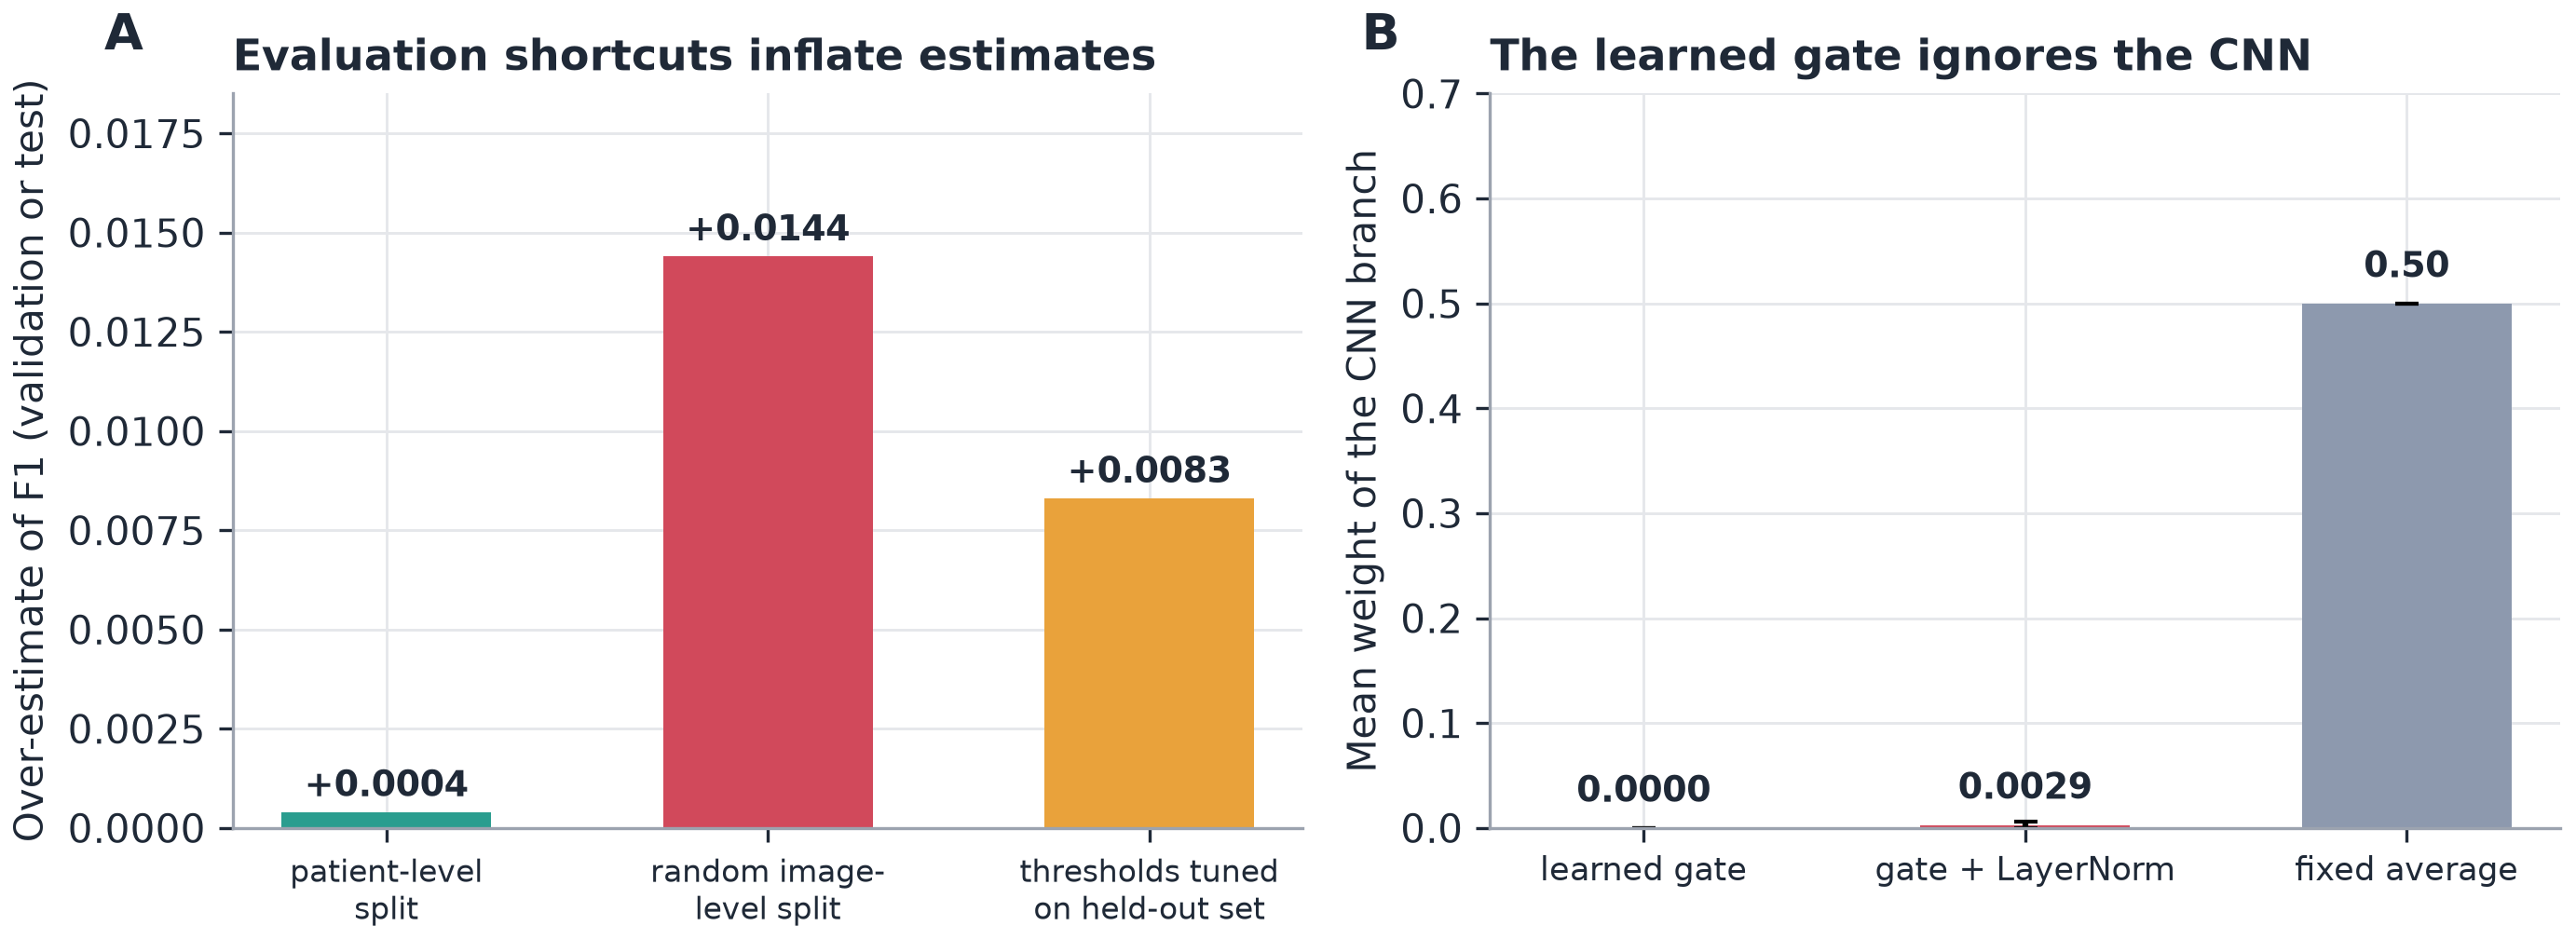
\includegraphics[width=1.0\textwidth]{fig7_leakage_and_gate.png}\caption{(A) How much a random image-level split and tuning thresholds on the held-out set overstate the score. (B) Mean weight the learned fusion gates give the CNN branch, compared with a fixed average.}\label{fig:7}\end{figure}\suppressfloats[t]

\subsection{Ablations (Table 5)}
Against the reference Swin-T (0.9089 [0.8576, 0.9509]) no configuration differed significantly. Heavy augmentation changed F1 by -0.0075 (p = 0.088), dropping the softmax head by -0.0051 (p = 0.152), two other seeds by +0.0055 and +0.0065 (p = 0.37 and 0.27), DenseNet121 by +0.0111 (p = 0.119), the CNN-only fusion branch by +0.0117 (p = 0.097) and the average of three seeds by +0.0049 (p = 0.38). All 95 \% intervals include zero. The seed-to-seed spread (0.9089 to 0.9154) is as large as most of these effects, so a single-run difference of this size should not be called an improvement (Fig. 8).

\setcounter{table}{4}
\begin{table}[!ht]\centering\small
\caption{Ablations (5 CV folds each, same held-out set; paired patient bootstrap vs. the reference)}\label{tab:ablation}
\resizebox{\ifdim\width>\textwidth\textwidth\else\width\fi}{!}{\begin{tabular}{lccccc}
\toprule
\textbf{config} & \textbf{held-out sample-F1 [95\% CI]} & \textbf{macro-F1} & \textbf{OOF - held-out} & \textbf{diff vs reference [95\% CI]} & \textbf{p} \\
\midrule
swin\_tiny\_s224 & 0.9089 [0.8576, 0.9509] & 0.837 & 0.0004 &  &  \\
swin\_tiny\_s224\_heavy & 0.9013 [0.8494, 0.9440] & 0.829 & 0.0074 & -0.0075 [-0.0164, 0.0009] & 0.088 \\
swin\_tiny\_s224\_ce0 & 0.9038 [0.8529, 0.9470] & 0.8261 & 0.0041 & -0.0051 [-0.0124, 0.0016] & 0.152 \\
swin\_tiny\_s224\_ce1 & 0.9132 [0.8616, 0.9568] & 0.8495 & 0.0012 & 0.0043 [-0.0063, 0.0149] & 0.447 \\
swin\_tiny\_s224\_leaky & 0.9163 [0.8644, 0.9587] & 0.856 & 0.0144 & 0.0074 [-0.0020, 0.0178] & 0.141 \\
swin\_tiny\_s224\_seed1 & 0.9143 [0.8620, 0.9576] & 0.8533 & 0.0028 & 0.0055 [-0.0060, 0.0173] & 0.366 \\
swin\_tiny\_s224\_seed2 & 0.9154 [0.8635, 0.9592] & 0.8585 & -0.0014 & 0.0065 [-0.0049, 0.0178] & 0.268 \\
hybrid\_gate\_s224 & 0.9136 [0.8609, 0.9568] & 0.8497 & 0.0000 & 0.0047 [-0.0063, 0.0161] & 0.401 \\
hybrid\_gate\_ln\_s224 & 0.9158 [0.8641, 0.9577] & 0.8536 & -0.0019 & 0.0069 [-0.0032, 0.0182] & 0.226 \\
hybrid\_avg\_s224 & 0.9164 [0.8651, 0.9585] & 0.8537 & -0.0004 & 0.0075 [-0.0048, 0.0201] & 0.235 \\
hybrid\_cnn\_s224 & 0.9205 [0.8684, 0.9613] & 0.8705 & -0.0012 & 0.0117 [-0.0016, 0.0257] & 0.097 \\
hybrid\_swin\_s224 & 0.9127 [0.8611, 0.9565] & 0.8467 & 0.0013 & 0.0038 [-0.0070, 0.0145] & 0.539 \\
densenet121\_s256 & 0.9200 [0.8694, 0.9618] & 0.8542 & -0.0042 & 0.0111 [-0.0022, 0.0275] & 0.119 \\
convnext\_tiny\_s256 & 0.9117 [0.8605, 0.9546] & 0.8472 & 0.0081 & 0.0028 [-0.0084, 0.0142] & 0.674 \\
swin\_3seeds\_average & 0.9137 [0.8623, 0.9574] & 0.848 & 0.0012 & 0.0049 [-0.0052, 0.0148] & 0.38 \\
\bottomrule
\end{tabular}}
\par\smallskip{\footnotesize \texttt{OOF - held-out} large and positive = the validation score over-estimates (compare \texttt{\_leaky} with the patient-level reference for the split ablation).}
\end{table}


\begin{figure}[t]\centering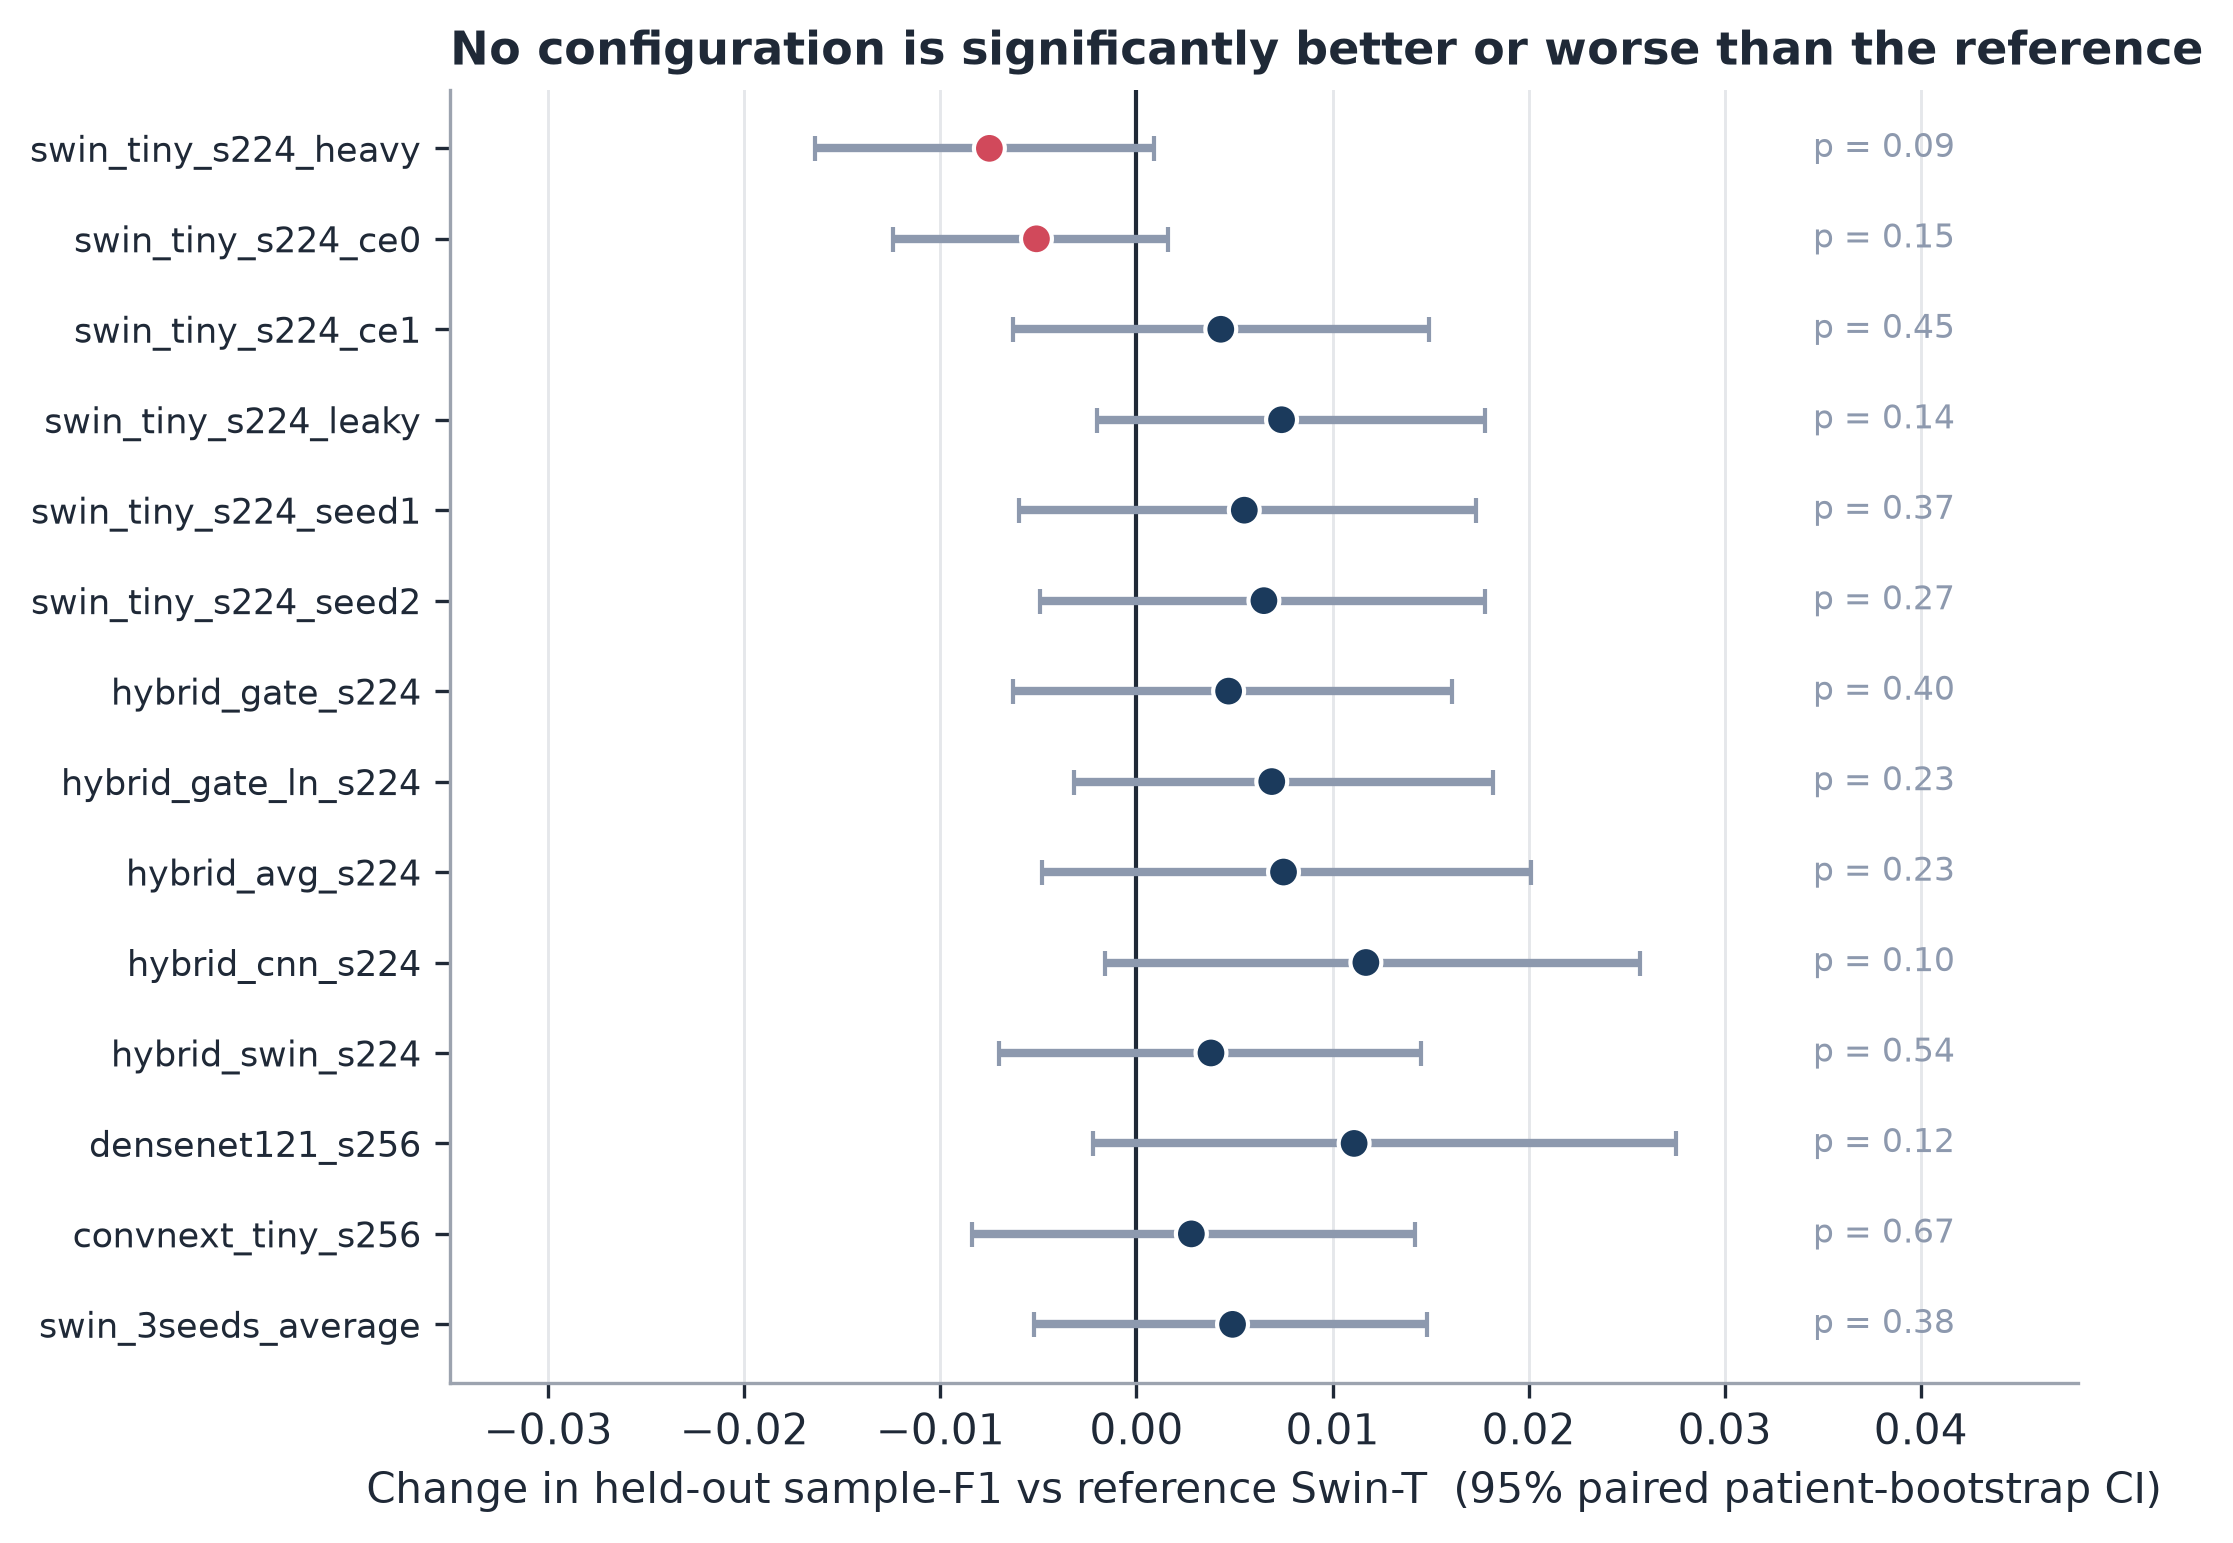
\includegraphics[width=0.9\textwidth]{fig2_ablation_forest.png}\caption{Change in held-out sample-F1 against the reference Swin-T for each ablation (95 \% paired patient-bootstrap interval; p-values on the right). None of the intervals excludes zero.}\label{fig:8}\end{figure}\suppressfloats[t]

\subsection{Fusion gate (Supplementary Table S3)}
Across five folds the learned gate gave the CNN branch a mean weight of 0.0000 (raw gate) and 0.0029 (LayerNorm gate). The fused model therefore behaves like the Transformer alone (Fig. 7B). Neither gate beat the fixed average (+0.0047 and +0.0069 against the reference, p = 0.40 and 0.23) or the CNN-only branch.

\subsection{Frozen foundation-model baseline}
A linear probe on frozen DINOv2-S reached 0.8699 OOF and 0.8859 on the held-out set [0.8327, 0.9318]. DINOv2-B reached 0.8839 [0.8300, 0.9276] and the ImageNet Swin-T 0.8762 [0.8248, 0.9204], while the fine-tuned Swin-T reference reached 0.9089. Frozen features therefore recover most of the fine-tuned performance, but not all of it. With 10 \% of the training patients the DINOv2-S probe scored 0.6435 OOF, with 25 \% 0.7457, with 50 \% 0.8235 and with all of them 0.8699. The curve is still rising, so this task looks limited by labelled data. A random-weight ResNet18 control gave 0.563 OOF but 0.095 on the held-out set, an inconsistency we could not resolve, so we leave it out of our claims. BiomedCLIP could not be downloaded and one ConvNeXt tag was invalid; both were skipped (Fig. 9).

\begin{figure}[t]\centering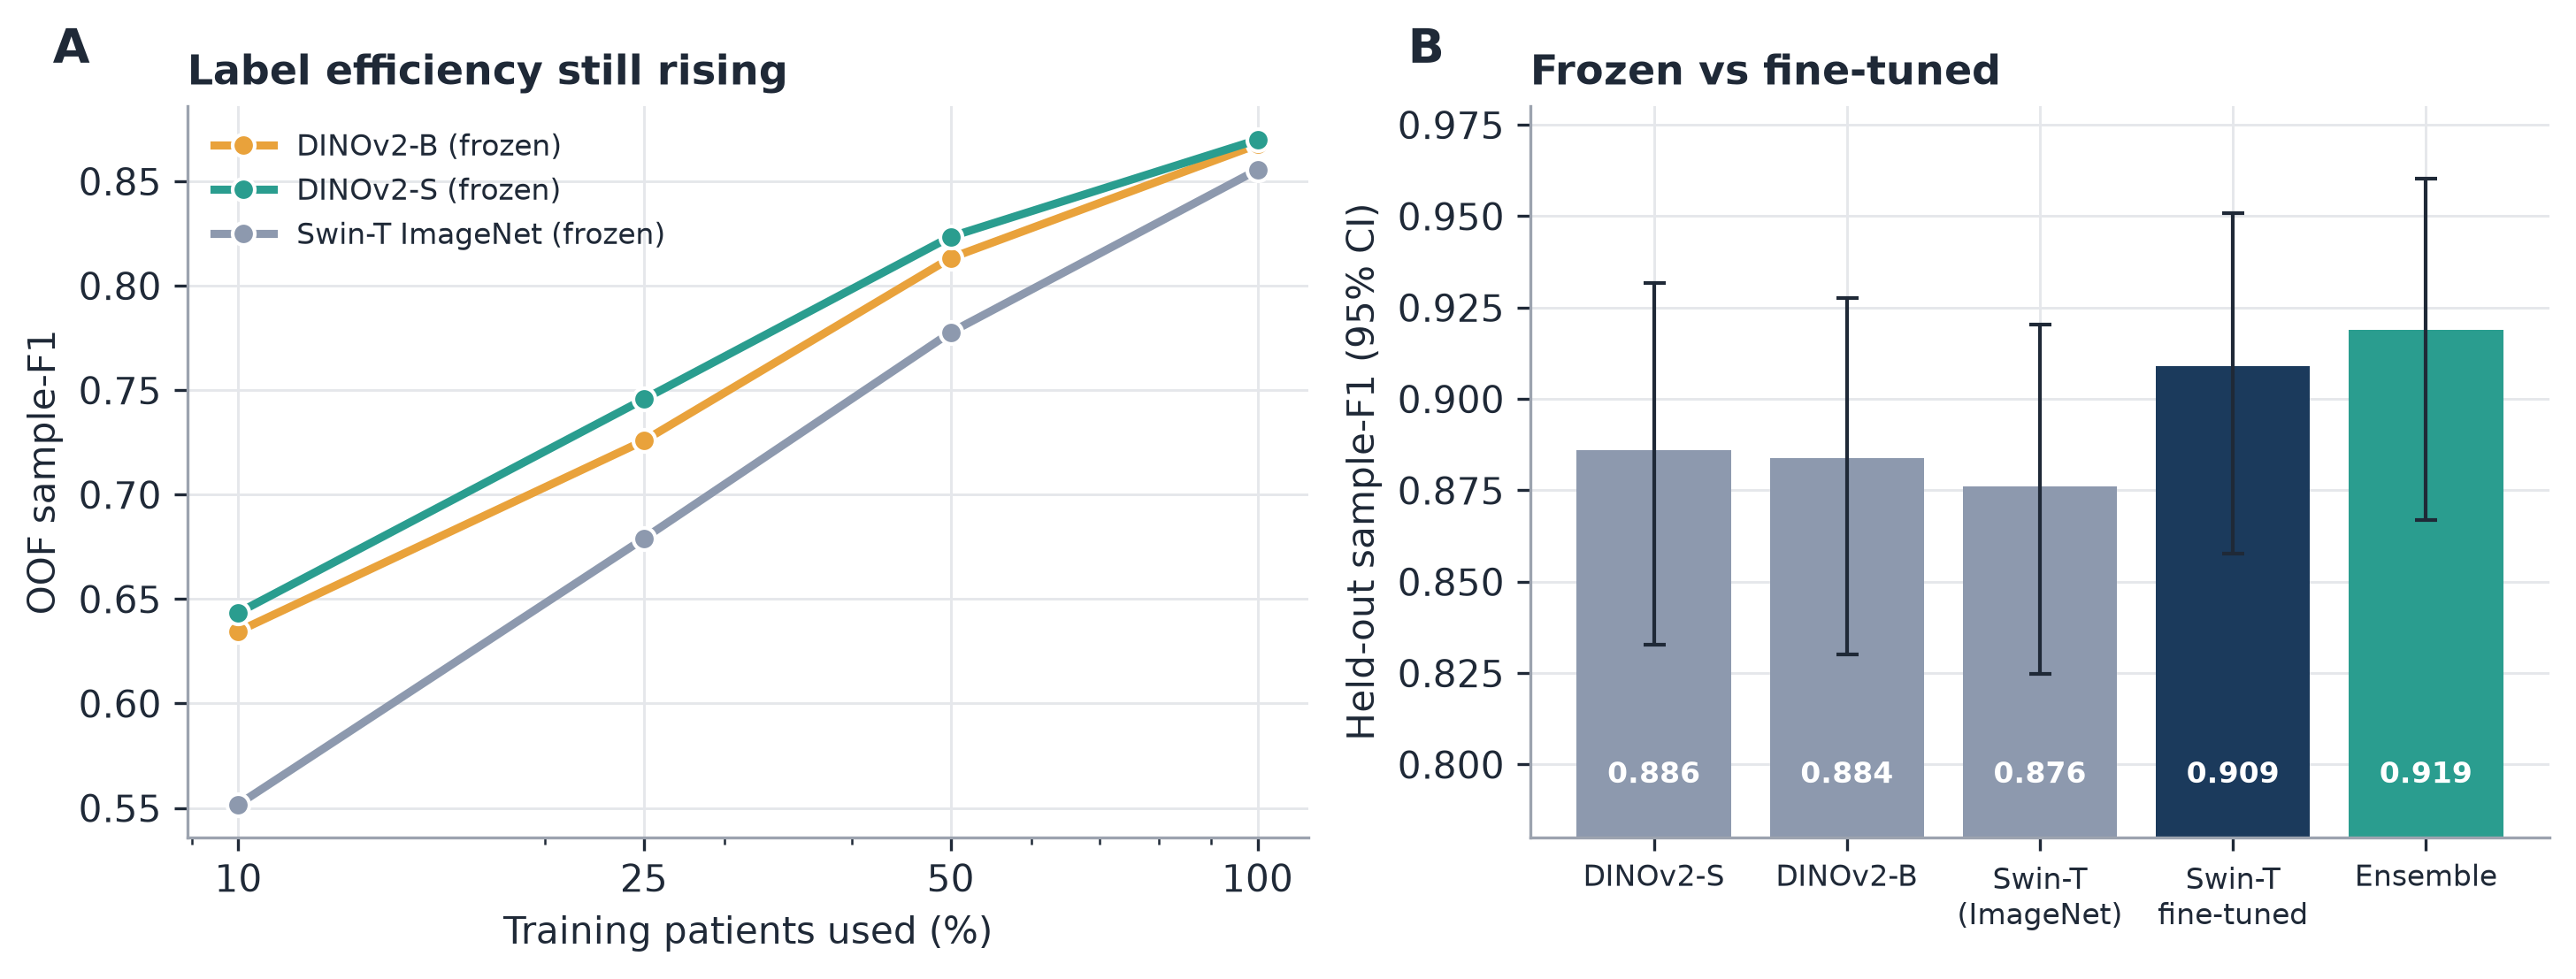
\includegraphics[width=1.0\textwidth]{fig5_foundation_models.png}\caption{(A) Label efficiency of frozen encoders. (B) Held-out F1 of the frozen probes next to the fine-tuned models.}\label{fig:9}\end{figure}\suppressfloats[t]

\subsection{Reliability and label audit}
\textbf{Calibration.} Top-1 accuracy of the five-model ensemble on the held-out set was 0.9257. ECE was 0.0545, and 0.0517 after temperature scaling (T = 1.15), so the ensemble is already close to calibrated and scaling changes little.

\textbf{Selective prediction.} Accuracy on the images the model kept rose from 0.926 at full coverage to 0.945 [0.900, 0.985] at 90 \% coverage, 0.973 at 80 \% and 0.982 at 70 \%. A threshold chosen on OOF predictions for 0.95 accuracy gave 0.937 accuracy at 98.5 \% coverage on the held-out set, so the target was missed. A 0.98 target gave 0.983 at 74 \% coverage. Operating points chosen on OOF predictions therefore do not transfer exactly (Fig. 10).


\textbf{Per class (held-out).} Chest reached an F1 of 0.993 (n = 138), and Cervical Spine, Feet, Hand, Sinus, Skull and Thigh reached 1.0. The weakest classes were Others (recall 0.41 [0.13, 0.91]), Forearm (0.33), Hip (0.33), Shoulder (0.60) and Ankle (0.75), all with 3 to 22 positives and wide intervals (Supplementary Table S7 and Supplementary Fig. S1).

\begin{figure}[t]\centering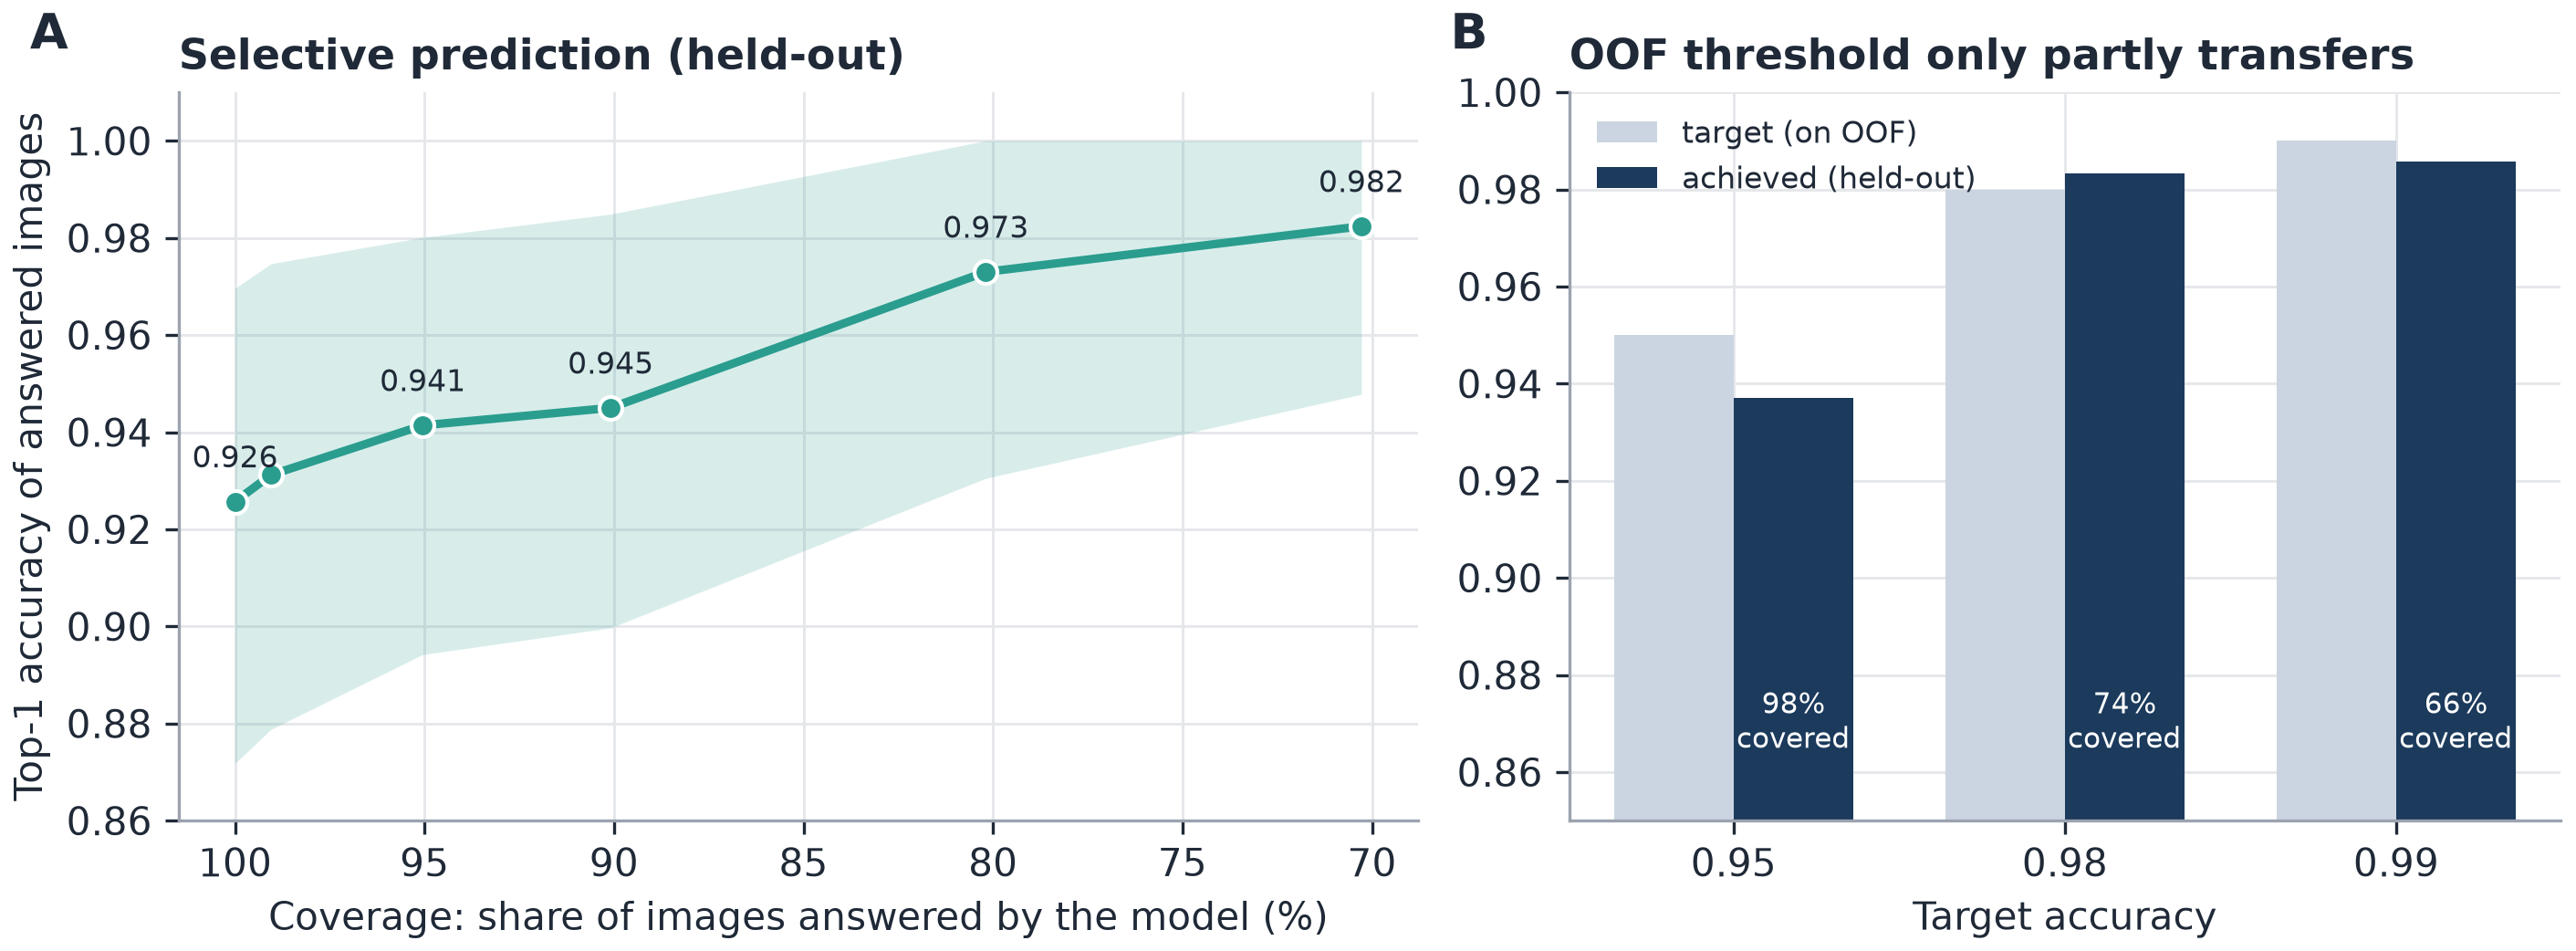
\includegraphics[width=0.8\textwidth]{fig4_reliability.png}\caption{(A) Accuracy on the images the model answers, as a function of coverage. (B) Accuracy targets chosen on out-of-fold predictions, and the accuracy reached on the held-out set.}\label{fig:10}\end{figure}\suppressfloats[t]



\begin{figure}[t]\centering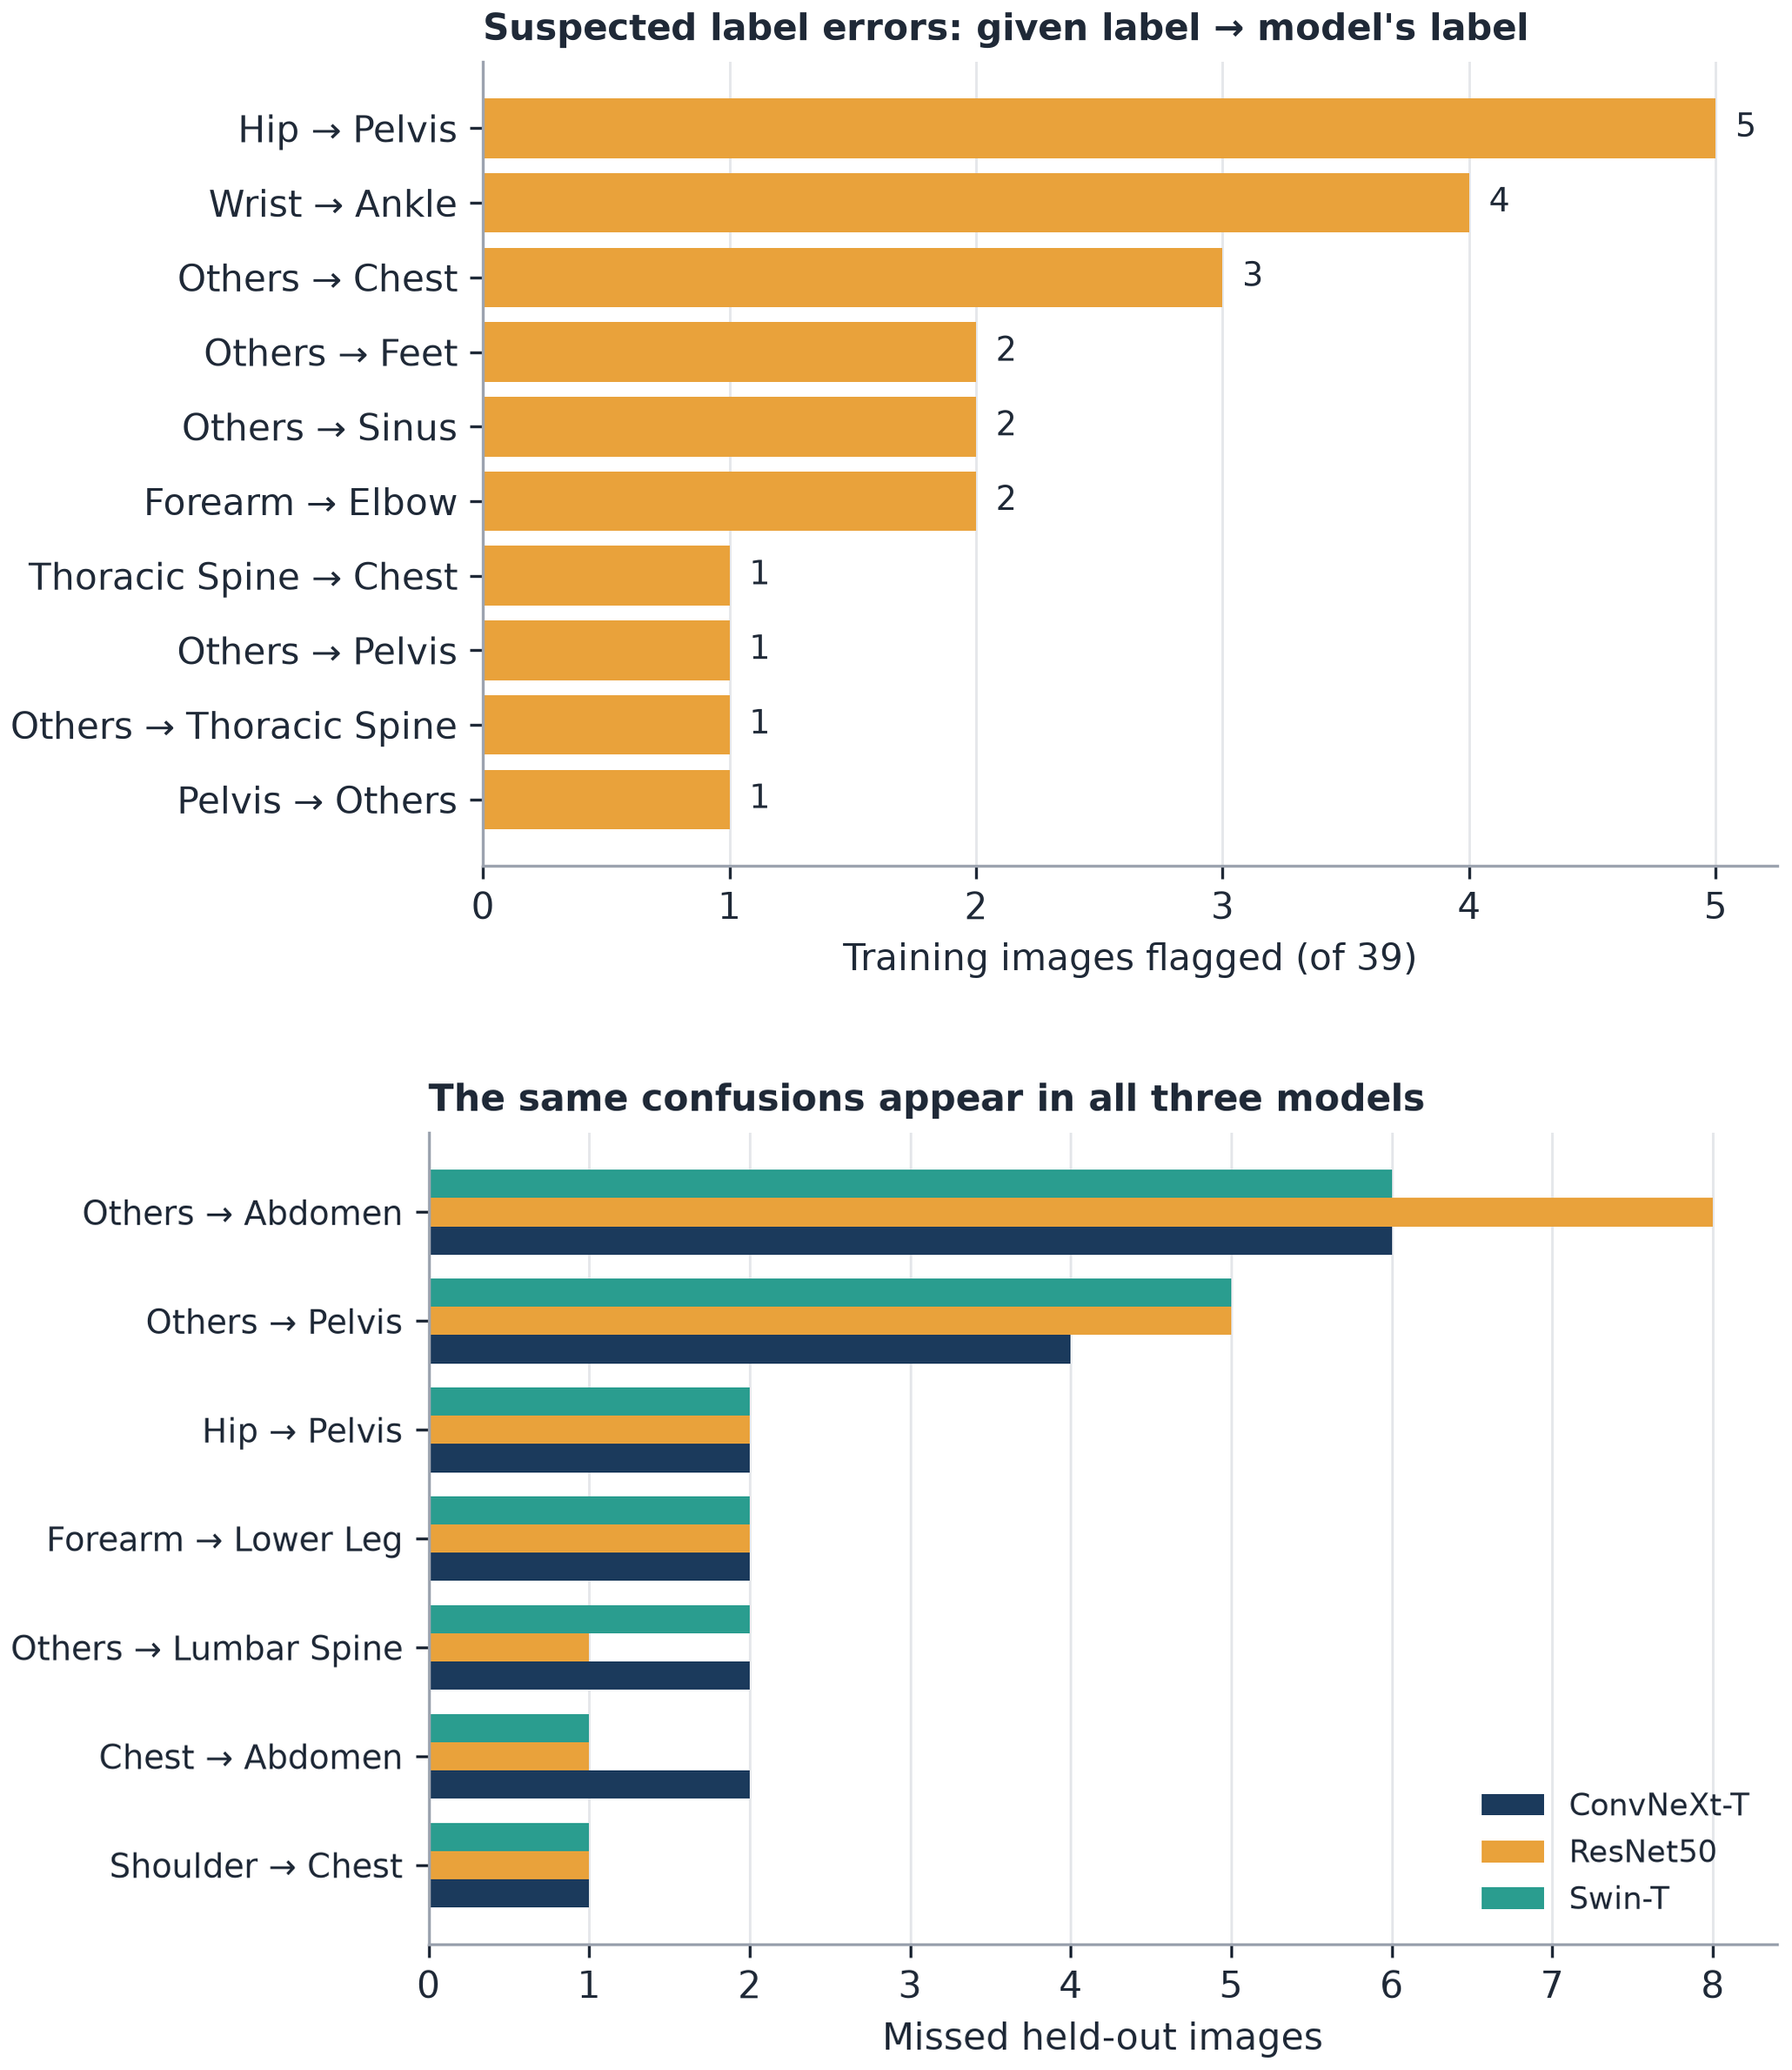
\includegraphics[width=1.0\textwidth]{c2_audit_confusions.png}\caption{(A) The pairs of given and suggested labels among the 39 suspected label errors. (B) The most frequent misclassifications of the three explained models on the held-out set.}\label{fig:11}\end{figure}\suppressfloats[t]
\textbf{Label audit.} At p of 0.9 or more, 39 of 1,415 training images (2.8 \%) were flagged. The most frequent pairs were Hip to Pelvis (5), Wrist to Ankle (4) and Others to Chest (3). The Hip-to-Pelvis pattern mirrors the low Hip recall, which fits either label noise or a real boundary problem between the two classes. No clinician has reviewed any of the 39 suspects.


\textbf{Error analysis (Supplementary Table S6).} In the three explained fold-0 models the most frequent held-out misses were Others labelled as Abdomen (6 to 8 images per model) and Others labelled as Pelvis (4 to 5), followed by Hip as Pelvis (2 per model) and Forearm as Lower Leg (2 per model). The heterogeneous "Others" class is mostly absorbed by large body regions. Fig. 11 shows which label pairs the suspects fall into (A) and how the three explained models misclassify the held-out images (B).



\subsection{Generalisation (Table 6 and Table 7; Supplementary Table S4)}
On the official MURA split the five-fold bagged ensemble reached an accuracy of 0.9747 [0.9663, 0.9818] and a macro-F1 of 0.9707 [0.9616, 0.9788]. Shah et al. (2026) report 0.9643 and 0.9574 on the same 3,197-image validation set, so the two results are comparable in data but not in method details.

On COVID-19 Radiography (4 classes, image-level split) sample-F1 was 0.9647 [0.9595, 0.9697] and macro-F1 0.9681, and these numbers may be optimistic.

Zero-shot transfer (Table 7) gave 0.875 to 0.880 from MURA to UNIFESP (n = 184) and 0.813 to 0.821 from UNIFESP to MURA (n = 12,000). From MURA to FracAtlas, restricted to hand and shoulder (1,281 of the 1,382 images are hand), accuracy was 0.691 with the softmax head and 0.858 with the sigmoid head. From UNIFESP to FracAtlas (hand, hip, leg, shoulder; n = 3,685) it was 0.708 and 0.698. Many FracAtlas JPEGs are truncated and were decoded only partly. Fig. 12 summarises the MURA comparison (A) and the transfer results (B).

\setcounter{table}{4}
\begin{table}[!ht]\centering\small
\caption{MURA body-part classification: held-out = MURA validation set}\label{tab:mura}
\resizebox{\textwidth}{!}{\begin{tabular}{lcc}
\toprule
\textbf{model} & \textbf{accuracy [95\% CI]} & \textbf{macro-F1 [95\% CI]} \\
\midrule
ours: 5-fold bagged ensemble (official MURA split) & 0.9747 [0.9663, 0.9818] & 0.9707 [0.9616, 0.9788] \\
Xception-Swin (Shah 2026) & 0.9643 (CI n/a) & 0.9574 (CI n/a) \\
DenseNet-201 & 0.9187 (CI n/a) & 0.9093 (CI n/a) \\
EfficientNet-B0 & 0.9043 (CI n/a) & 0.8952 (CI n/a) \\
ResNet-101 & 0.8934 (CI n/a) & 0.8831 (CI n/a) \\
VGG-19 & 0.8612 (CI n/a) & 0.8498 (CI n/a) \\
\bottomrule
\end{tabular}}
\par\smallskip{\footnotesize Shah et al. 2026 (Supplementary Table S4; verified in the full text): same MURA validation set (3,197 images), fixed seed 42, image-level evaluation; no CI is shown for these body-part numbers.}
\end{table}


\setcounter{table}{6}
\begin{table}[!ht]\centering\small
\caption{Zero-shot cross-dataset transfer through the class map}\label{tab:transfer}
\resizebox{\ifdim\width>\textwidth\textwidth\else\width\fi}{!}{\begin{tabular}{lccccccc}
\toprule
\textbf{source} & \textbf{target} & \textbf{head} & \textbf{groups} & \textbf{n} & \textbf{accuracy} & \textbf{95 \% CI} & \textbf{macro-F1} \\
\midrule
mura & unifesp & softmax & elbow,finger,forearm,hand,shoulder,wrist & 184 & 0.875 & [0.826, 0.924] & 0.8478 \\
mura & unifesp & sigmoid & elbow,finger,forearm,hand,shoulder,wrist & 184 & 0.8804 & [0.837, 0.924] & 0.856 \\
unifesp & mura & softmax & elbow,finger,forearm,hand,shoulder,wrist & 12000 & 0.8133 & [0.806, 0.820] & 0.7444 \\
unifesp & mura & sigmoid & elbow,finger,forearm,hand,shoulder,wrist & 12000 & 0.8208 & [0.814, 0.828] & 0.7481 \\
mura & fracatlas & softmax & hand,shoulder & 1382 & 0.691 & [0.667, 0.715] & 0.5606 \\
mura & fracatlas & sigmoid & hand,shoulder & 1382 & 0.8575 & [0.840, 0.875] & 0.7115 \\
unifesp & fracatlas & softmax & hand,hip,leg,shoulder & 3685 & 0.708 & [0.693, 0.722] & 0.7409 \\
unifesp & fracatlas & sigmoid & hand,hip,leg,shoulder & 3685 & 0.6982 & [0.684, 0.713] & 0.699 \\
\bottomrule
\end{tabular}}
\par\smallskip{\footnotesize Closed-set decision among the shared groups; CIs are image-level (the targets have no patient ids). The class map is an assumption to be checked by a clinician.}
\end{table}


\begin{figure}[t]\centering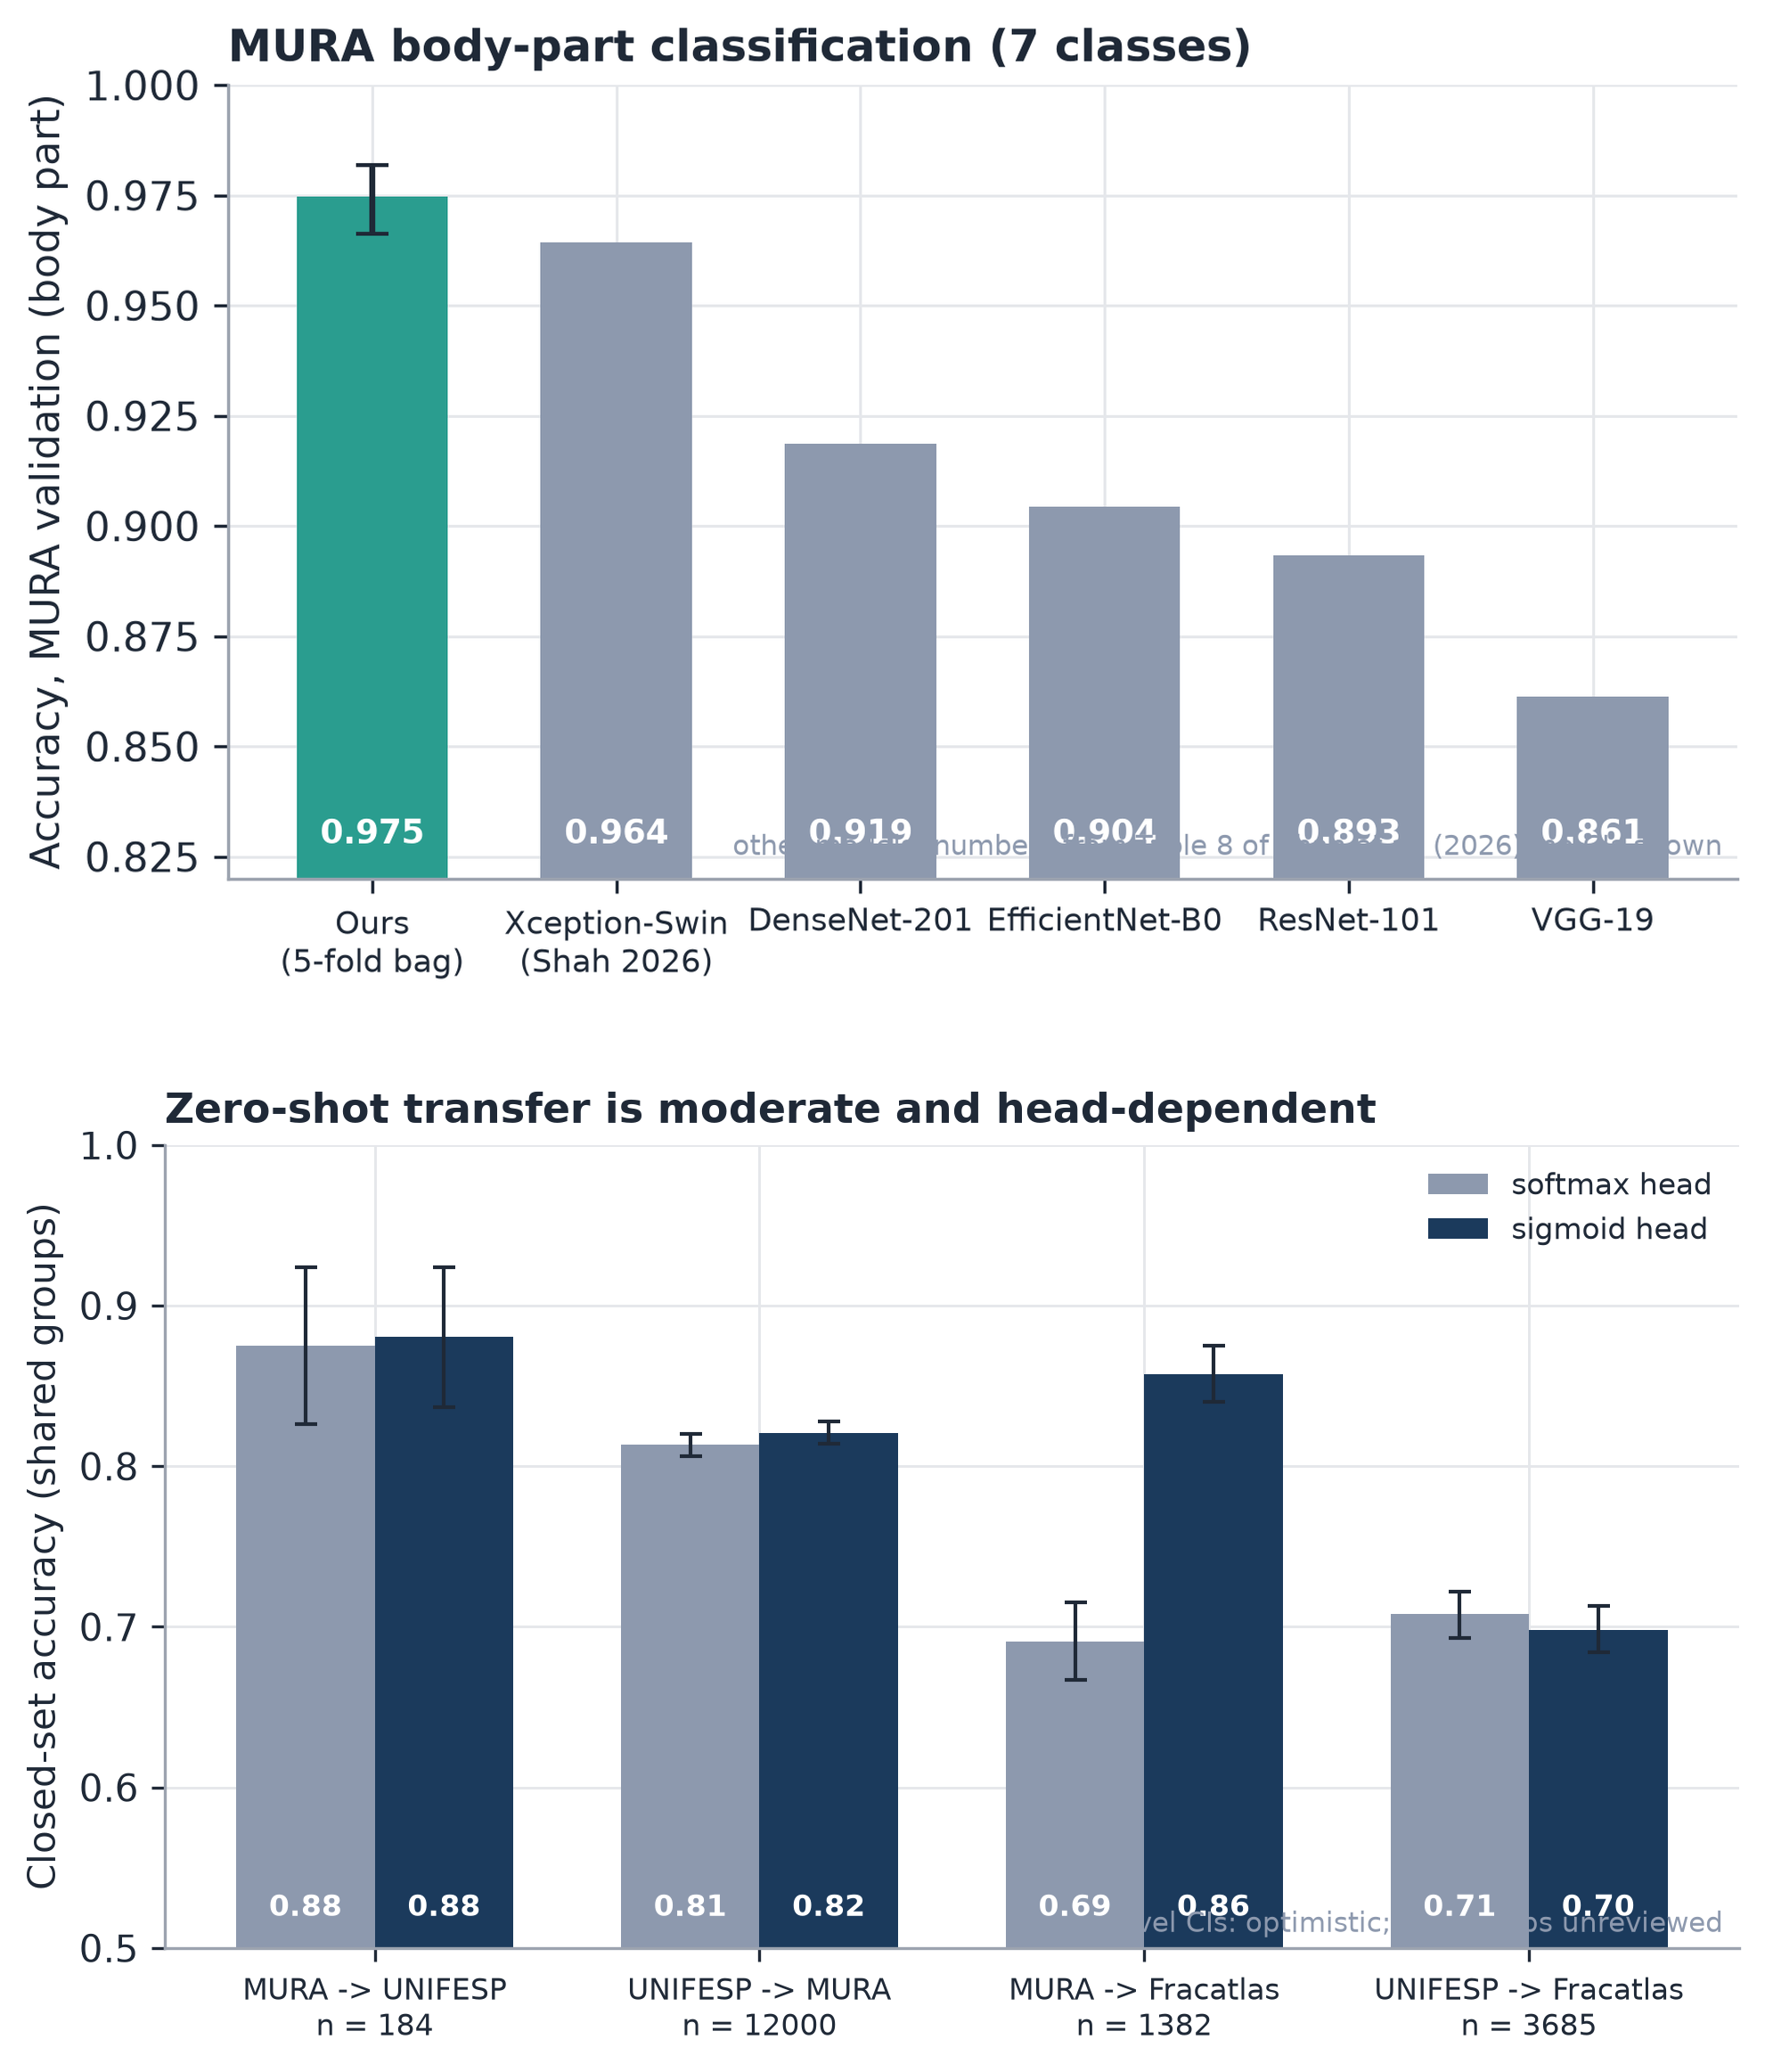
\includegraphics[width=1.0\textwidth]{c3_mura_transfer.png}\caption{(A) Body-part accuracy on MURA (seven classes), compared with the models reported by Shah et al. (2026). (B) Zero-shot accuracy through the class map, for the softmax and sigmoid heads; intervals come from an image-level bootstrap and are optimistic.}\label{fig:12}\end{figure}\suppressfloats[t]
Transfer is moderate and depends on the head, and the class maps are our own assumptions.


\subsection{Explainability (Supplementary Table S5)}
For all three models, deleting the most salient pixels first removed class evidence faster than deleting a random block of the same size (gain 0.284 [0.252, 0.316] for ConvNeXt-T, 0.204 for ResNet50, 0.164 for Swin-T). The maps were uncorrelated with those of randomly initialised networks for ConvNeXt-T and Swin-T (rho 0.11 and 0.02). ResNet50 differed too, but with a systematic negative correlation (rho -0.31). The feature grids are coarse (7 $\times$ 7 to 8 $\times$ 8), there is no localisation ground truth and no radiologist reviewed the maps. We therefore describe them as faithful to the model, not as clinically valid (Fig. 13).

\begin{figure}[t]\centering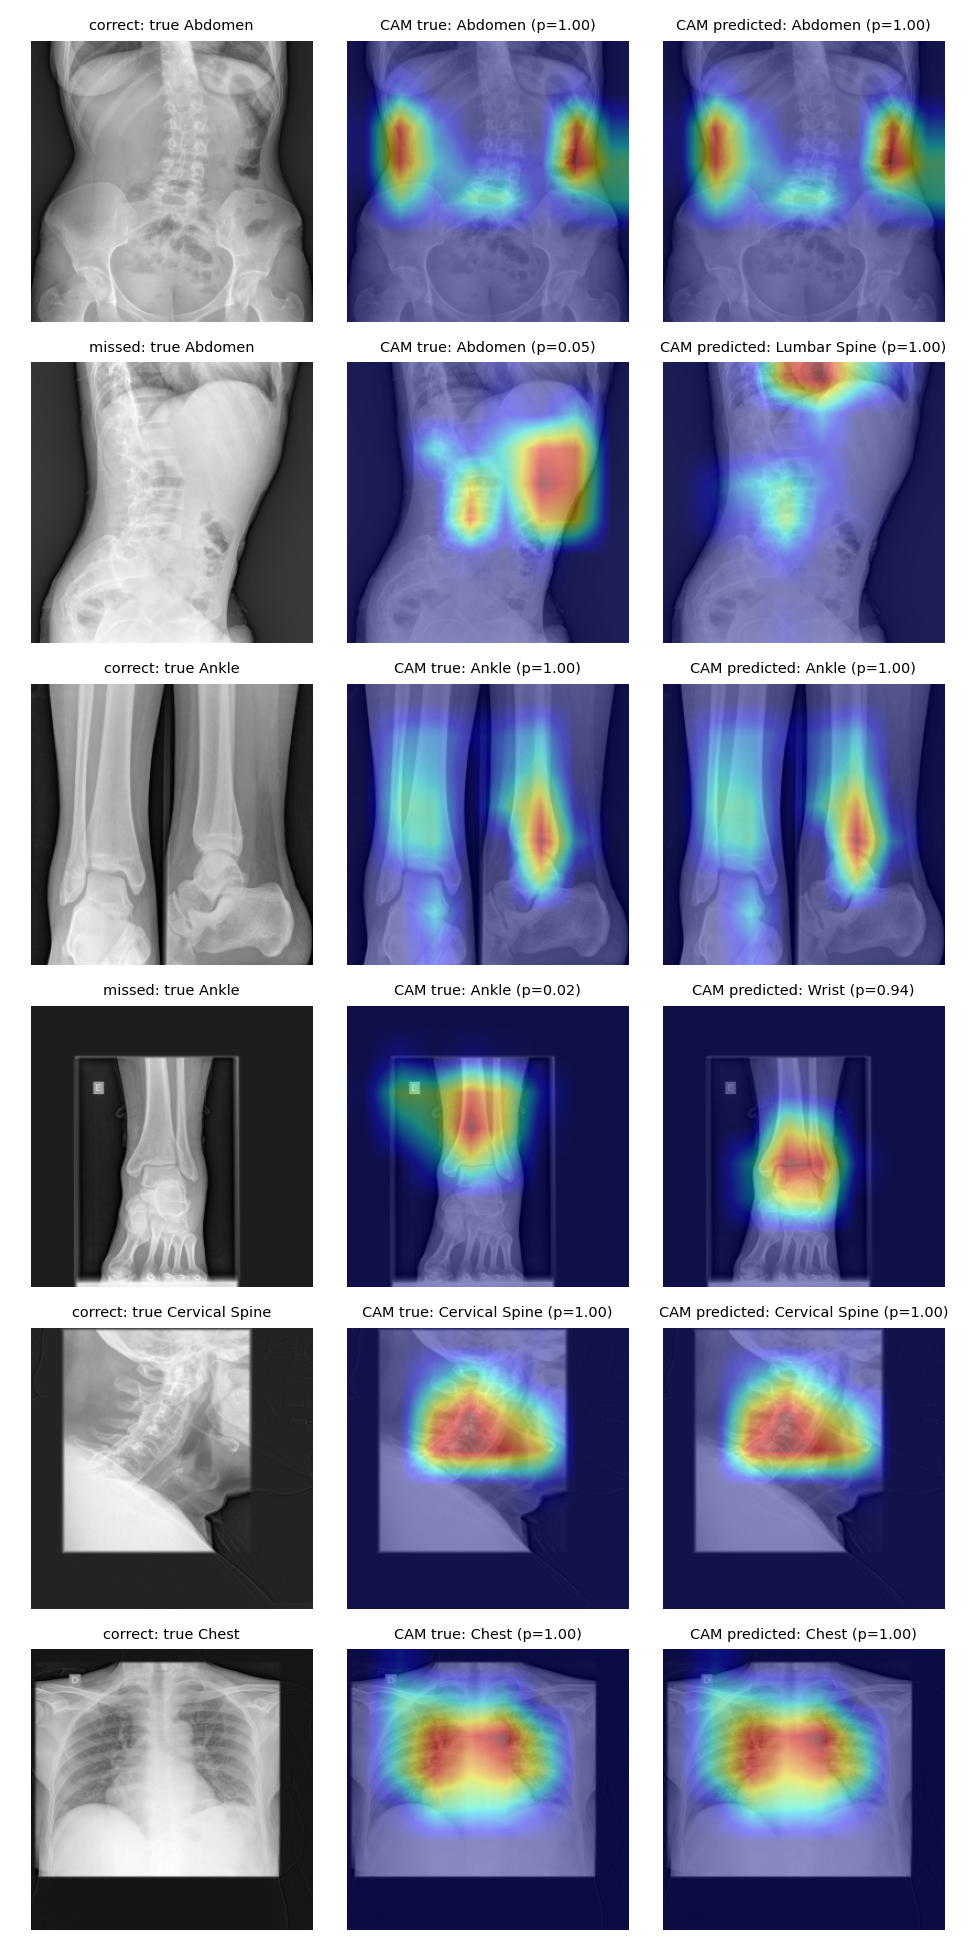
\includegraphics[width=0.325\textwidth]{gradcam_gallery_1.png}\hfill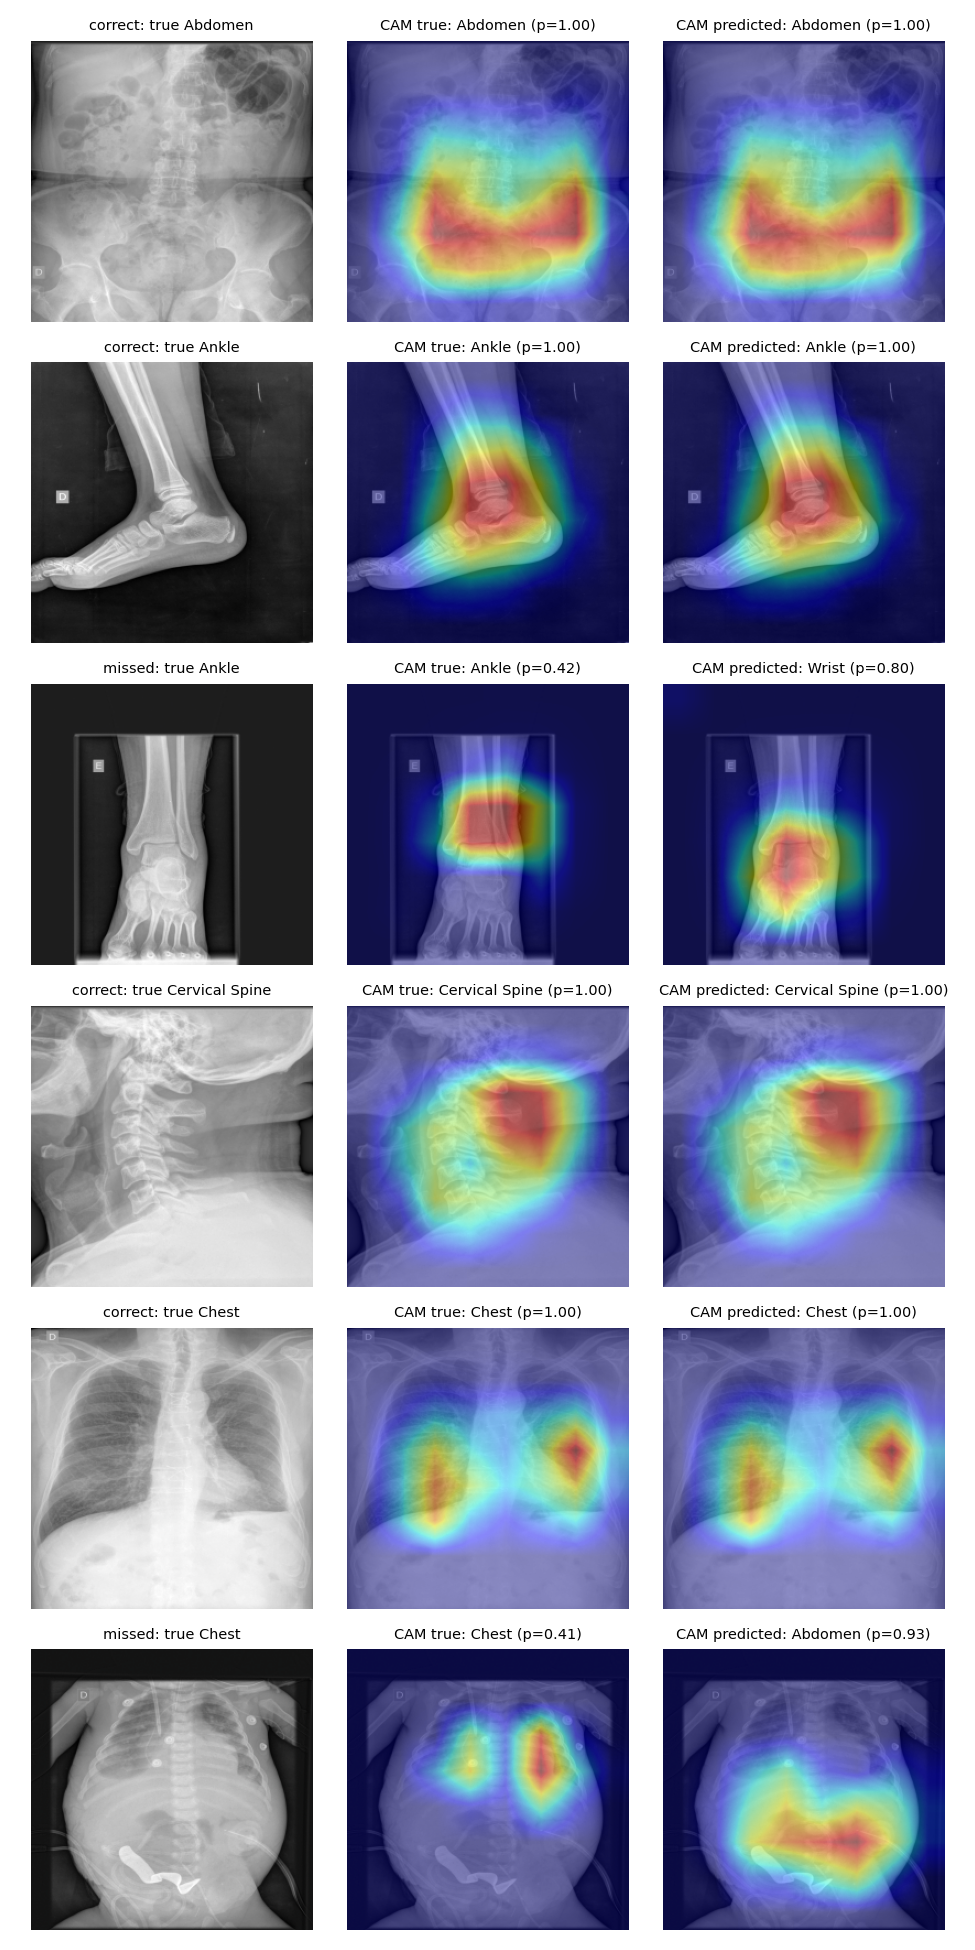
\includegraphics[width=0.325\textwidth]{gradcam_gallery_2.png}\hfill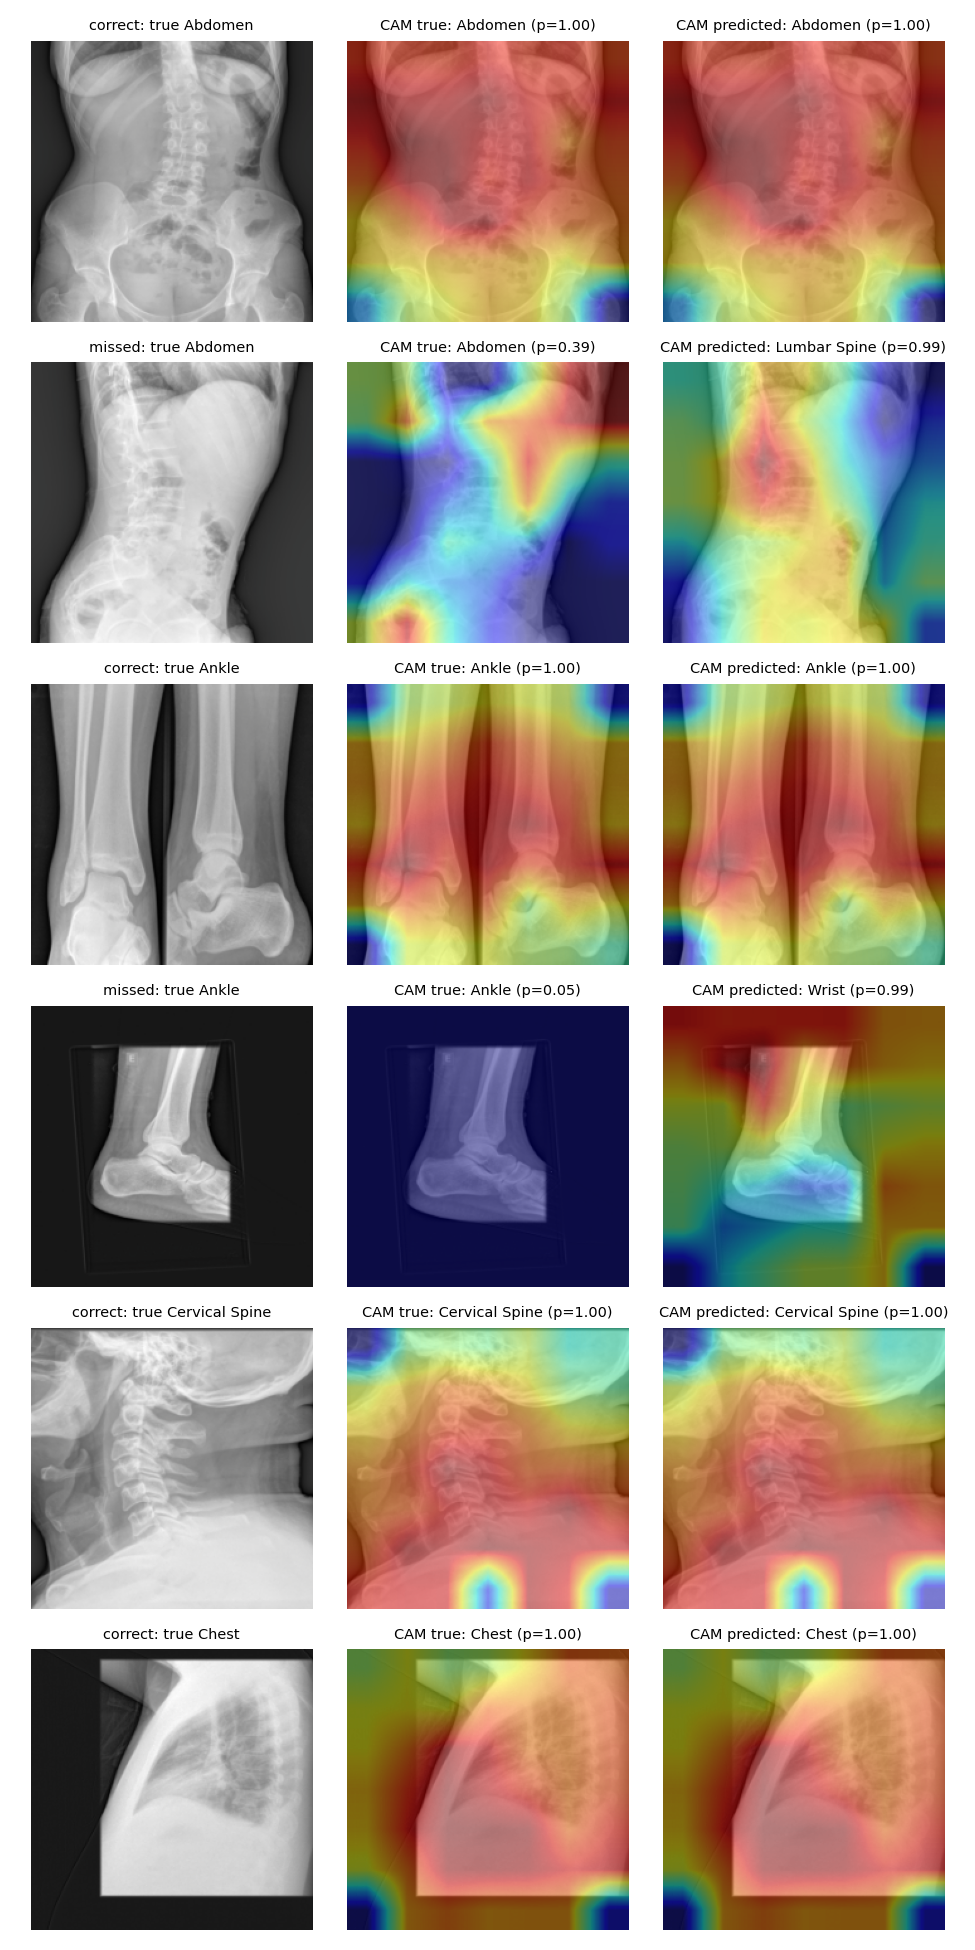
\includegraphics[width=0.325\textwidth]{gradcam_gallery_3.png}\caption{Grad-CAM galleries for ConvNeXt-T (left), ResNet50 (middle) and Swin-T (right). For each class there is one correct and one missed held-out image, with the map for the true class and for the predicted class.}\label{fig:13}\end{figure}\suppressfloats[t]





\section{Discussion}
Evaluation mattered more than architecture here. Ensembling, fusion, heavy augmentation, extra seeds and pseudo-labelling each moved the held-out score by about 0.01 at most, none of them significantly, and seed noise was about as large. Papers that report differences of this size without intervals deserve some caution.
Most errors sit in the rare classes (1 to 6 held-out positives) and in the heterogeneous "Others" class. The Hip-to-Pelvis cluster in the audit, and the competition hosts' offline re-annotation of the test set, suggest that label noise sets part of the ceiling, as Langer et al. (2024) found on a hospital dataset. The label-efficiency curve was still rising, so more labelled data would probably help more than a different architecture.
We did not test why the gate collapsed. One possibility is that a gate learned on the raw features of two networks with different activation scales lets one branch dominate. The learned weights point to a degenerate solution, not to complementary fusion, and fixed averaging was no worse.
For clinical use, a router that answers 90 \% of the images keeps 94.5 \% top-1 accuracy and sends the other 10 \% to a person. The operating point chosen on OOF predictions should be re-validated on local data before anyone relies on it. We see the classifier as a way to flag suspicious metadata, not as a replacement for it.
Our MURA accuracy is higher than the one published figure we found for this task. Other studies report 97 to 99 \% on other data and with much larger private training sets (Langer et al. 2024; Mitsuyama et al. 2026), and we do not claim to outperform them.


\section{Limitations}
The dataset comes from a single centre and has 1,738 labelled images, and the held-out set of 323 images has only 1 to 6 positives for several classes. The COVID and FracAtlas results use image-level splits and intervals. The class maps used for transfer are ours and nobody has reviewed them, and neither the label audit nor the Grad-CAM maps have been checked by a clinician. The private test labels are noisy. Stage 2 uses unlabelled test images (a transductive step) and weights fitted on OOF predictions. The explainability analysis covers one fold per model. The results come from several Kaggle accounts, although all of them can be reproduced from the released code. One control (the random-weight probe) was inconsistent and is excluded. We did not record a full package list for the Kaggle runs, and we had no external clinical site.



\section{Conclusion}
A carefully evaluated ensemble reaches a sample-F1 of 0.919 (0.867 to 0.960) on public UNIFESP data, and fusion, extra seeds and pseudo-labels bring no significant benefit. Random splits and test-set thresholds inflate the estimates. MURA body-part classification reaches about 97 \% accuracy on the official validation set. The model is reasonably calibrated, supports selective prediction, and surfaces a small set of suspected label errors that experts should look at.


\section{Declarations}
\emph{Funding:} This research did not receive any specific grant from funding agencies in the public, commercial, or not-for-profit sectors.
\emph{Declaration of competing interest:} none declared.
\emph{CRediT authorship contribution statement:} Sheikh Noor Abdullah: Conceptualization, Methodology, Software, Formal analysis, Investigation, Data curation, Visualization, Writing - original draft. A.B.M. Kabir Hossain: Supervision, Writing - review and editing. The corresponding author is Sheikh Noor Abdullah.
\emph{Ethics:} only public, de-identified datasets were used (UNIFESP CC BY-NC-SA 4.0, non-commercial; FracAtlas CC BY 4.0; MURA under the Stanford University School of Medicine Dataset Research Use Agreement; COVID-19 Radiography files (c) original authors).
\emph{Data availability:} all datasets used are public, with access conditions given in Section 3 (MURA requires AIMI membership and acceptance of a non-commercial research use agreement, and MURA images cannot be redistributed). The code, split lists, seeds, result files and figure scripts are deposited at [GitHub repository and Zenodo DOI to be inserted]; the third-party datasets themselves cannot be re-deposited because of their licences.
\emph{CLAIM 2024 checklist:} to be completed.


\section{Declaration of generative AI and AI-assisted technologies in the manuscript preparation process}
During the preparation of this work the authors used Claude (Anthropic) to help write analysis code, generate figures and tables from the result files, and draft and edit text. After using this tool, the authors reviewed and edited the content as needed, checked every reported number against the result files, and take full responsibility for the content of the published article.


\bibliographystyle{plainnat}\bibliography{refs}
\clearpage\appendix
\section{Tables}
\setcounter{table}{0}
\Needspace*{9\baselineskip}
\begin{center}\begin{minipage}{\textwidth}\small
\captionof{table}{UNIFESP held-out performance (decisions made on out-of-fold predictions only)}\label{tab:main}
\resizebox{\textwidth}{!}{\begin{tabular}{lcccc}
\toprule
\textbf{decoding} & \textbf{sample-mean F1} & \textbf{macro-F1} & \textbf{micro-F1} & \textbf{subset acc.} \\
\midrule
ensemble, threshold 0.5 & 0.9164 & 0.8537 & 0.9130 & 0.8885 \\
ensemble, 0.5 + min-one & 0.9164 & 0.8537 & 0.9130 & 0.8885 \\
ensemble, per-class thresholds tuned on OOF + min-one & 0.9189 [0.8669, 0.9602] & 0.8630 [0.6891, 0.8916] & 0.9148 & 0.8885 \\
best single run by OOF (convnext\_tiny\_s256), 0.5 + min-one & 0.9123 & 0.8482 & 0.9070 & 0.8762 \\
\bottomrule
\end{tabular}}
\par\smallskip{\footnotesize Held-out set: 323 images / 156 patients; 95 \% CIs by patient-level bootstrap. Ensemble minus best single: +0.0066 [-0.0002, +0.0142], p = 0.063. Ensemble weights (OOF, Caruana): efficientnetv2\_s\_s256 0.10, convnext\_tiny\_s256 0.27, resnet50\_s256\_heavy 0.29, efficientnet\_b3\_s256\_hv 0.34.}
\end{minipage}\end{center}
\setcounter{table}{0}
\Needspace*{9\baselineskip}
\begin{center}\begin{minipage}{\textwidth}\small
\captionof{table}{Single runs (head/TTA variant chosen on OOF)}\label{tab:runs}
\resizebox{\textwidth}{!}{\begin{tabular}{lccc}
\toprule
\textbf{run} & \textbf{chosen variant} & \textbf{oof chosen variant} & \textbf{holdout sample mean f1 0.5 min one} \\
\midrule
swin\_tiny\_s224 & blend & 0.9147 & 0.9133 \\
densenet121\_s256 & blend & 0.918 & 0.9221 \\
efficientnetv2\_s\_s256 & blend\_tta & 0.9186 & 0.9173 \\
convnext\_tiny\_s256 & blend\_tta & 0.9234 & 0.9123 \\
resnet50\_s256\_heavy & blend & 0.9064 & 0.9104 \\
efficientnet\_b3\_s256\_hv & blend\_tta & 0.9133 & 0.9172 \\
\bottomrule
\end{tabular}}
\par\smallskip{\footnotesize OOF = pooled out-of-fold sample-mean F1 of the chosen variant is in the full CSV.}
\end{minipage}\end{center}
\begin{table}[t]
\centering\small
\caption{Kaggle UNIFESP private score vs. the competition leaderboard}\label{tab:kaggle}
\resizebox{\textwidth}{!}{\begin{tabular}{lcc}
\toprule
\textbf{entry} & \textbf{private\_score} & \textbf{public\_score} \\
\midrule
\#1 Harshit Sheoran & 0.93378 &  \\
\#2 JGK (ResNet50/152, FastAI) & 0.92787 &  \\
ours: stage-2 union (late submission) & 0.92638 & 0.93378 \\
ours: stage-1 ensemble (late submission) & 0.92563 & 0.92704 \\
\#3 Colin Greeley & 0.92488 &  \\
\#4 KobeU Systems Medicine & 0.92414 &  \\
\#5 wangkui & 0.92182 &  \\
\bottomrule
\end{tabular}}
\par\smallskip{\footnotesize Mean F1 (sample-wise); private score uses \textasciitilde{}60 \% of the test set with the original (partly noisy) labels, so differences of \textasciitilde{}0.003 are within noise. Late submissions are not listed on the leaderboard; report ALL submissions made.}
\end{table}
\setcounter{table}{4}
\begin{table}[!ht]\centering\small
\caption{Ablations (5 CV folds each, same held-out set; paired patient bootstrap vs. the reference)}\label{tab:ablation}
\resizebox{\ifdim\width>\textwidth\textwidth\else\width\fi}{!}{\begin{tabular}{lccccc}
\toprule
\textbf{config} & \textbf{held-out sample-F1 [95\% CI]} & \textbf{macro-F1} & \textbf{OOF - held-out} & \textbf{diff vs reference [95\% CI]} & \textbf{p} \\
\midrule
swin\_tiny\_s224 & 0.9089 [0.8576, 0.9509] & 0.837 & 0.0004 &  &  \\
swin\_tiny\_s224\_heavy & 0.9013 [0.8494, 0.9440] & 0.829 & 0.0074 & -0.0075 [-0.0164, 0.0009] & 0.088 \\
swin\_tiny\_s224\_ce0 & 0.9038 [0.8529, 0.9470] & 0.8261 & 0.0041 & -0.0051 [-0.0124, 0.0016] & 0.152 \\
swin\_tiny\_s224\_ce1 & 0.9132 [0.8616, 0.9568] & 0.8495 & 0.0012 & 0.0043 [-0.0063, 0.0149] & 0.447 \\
swin\_tiny\_s224\_leaky & 0.9163 [0.8644, 0.9587] & 0.856 & 0.0144 & 0.0074 [-0.0020, 0.0178] & 0.141 \\
swin\_tiny\_s224\_seed1 & 0.9143 [0.8620, 0.9576] & 0.8533 & 0.0028 & 0.0055 [-0.0060, 0.0173] & 0.366 \\
swin\_tiny\_s224\_seed2 & 0.9154 [0.8635, 0.9592] & 0.8585 & -0.0014 & 0.0065 [-0.0049, 0.0178] & 0.268 \\
hybrid\_gate\_s224 & 0.9136 [0.8609, 0.9568] & 0.8497 & 0.0000 & 0.0047 [-0.0063, 0.0161] & 0.401 \\
hybrid\_gate\_ln\_s224 & 0.9158 [0.8641, 0.9577] & 0.8536 & -0.0019 & 0.0069 [-0.0032, 0.0182] & 0.226 \\
hybrid\_avg\_s224 & 0.9164 [0.8651, 0.9585] & 0.8537 & -0.0004 & 0.0075 [-0.0048, 0.0201] & 0.235 \\
hybrid\_cnn\_s224 & 0.9205 [0.8684, 0.9613] & 0.8705 & -0.0012 & 0.0117 [-0.0016, 0.0257] & 0.097 \\
hybrid\_swin\_s224 & 0.9127 [0.8611, 0.9565] & 0.8467 & 0.0013 & 0.0038 [-0.0070, 0.0145] & 0.539 \\
densenet121\_s256 & 0.9200 [0.8694, 0.9618] & 0.8542 & -0.0042 & 0.0111 [-0.0022, 0.0275] & 0.119 \\
convnext\_tiny\_s256 & 0.9117 [0.8605, 0.9546] & 0.8472 & 0.0081 & 0.0028 [-0.0084, 0.0142] & 0.674 \\
swin\_3seeds\_average & 0.9137 [0.8623, 0.9574] & 0.848 & 0.0012 & 0.0049 [-0.0052, 0.0148] & 0.38 \\
\bottomrule
\end{tabular}}
\par\smallskip{\footnotesize \texttt{OOF - held-out} large and positive = the validation score over-estimates (compare \texttt{\_leaky} with the patient-level reference for the split ablation).}
\end{table}
\setcounter{table}{1}
\begin{table}[!ht]\centering\small
\caption{Decoding ablation and evaluation leakage}\label{tab:decoding}
\resizebox{\ifdim\width>\textwidth\textwidth\else\width\fi}{!}{\begin{tabular}{p{0.64\textwidth}cc}
\toprule
\textbf{decoding} & \textbf{held-out sample-F1 [95\% CI]} & \textbf{macro-F1} \\
\midrule
0.5, empty allowed & 0.9058 [0.8544, 0.9480] & 0.8361 \\
0.5 + min-one & 0.9089 [0.8576, 0.9509] & 0.837 \\
global threshold 0.50 (tuned on OOF) + min-one & 0.9089 [0.8576, 0.9509] & 0.837 \\
per-class thresholds tuned on OOF (honest) + min-one & 0.9099 [0.8599, 0.9523] & 0.8413 \\
per-class thresholds tuned on HELD-OUT (leaky) + min-one & 0.9182 [0.8668, 0.9592] & 0.8565 \\
\bottomrule
\end{tabular}}
\par\smallskip{\footnotesize Leak gap (thresholds tuned on the held-out set minus thresholds tuned on OOF) = +0.0083.}
\end{table}
\setcounter{table}{2}
\begin{table}[!ht]\centering\small
\caption{Mean weight given to the CNN branch by the fusion gate (5 folds)}\label{tab:gate}
\resizebox{\ifdim\width>\textwidth\textwidth\else\width\fi}{!}{\begin{tabular}{p{0.38\textwidth}cccc}
\toprule
\textbf{config} & \textbf{mean} & \textbf{std} & \textbf{min} & \textbf{max} \\
\midrule
hybrid\_avg\_s224 & 0.5 & 0.0 & 0.5 & 0.5 \\
hybrid\_cnn\_s224 & 1.0 & 0.0 & 1.0 & 1.0 \\
hybrid\_gate\_ln\_s224 & 0.0029 & 0.003 & 0.0006 & 0.008 \\
hybrid\_gate\_s224 & 0.0 & 0.0 & 0.0 & 0.0001 \\
hybrid\_swin\_s224 & 0.0 & 0.0 & 0.0 & 0.0 \\
\bottomrule
\end{tabular}}
\par\smallskip{\footnotesize hybrid\_avg is fixed at 0.5; hybrid\_cnn / hybrid\_swin are 1 / 0 by construction.}
\end{table}

\setcounter{table}{4}
\begin{table}[!ht]\centering\small
\caption{MURA body-part classification: held-out = MURA validation set}\label{tab:mura}
\resizebox{\textwidth}{!}{\begin{tabular}{lcc}
\toprule
\textbf{model} & \textbf{accuracy [95\% CI]} & \textbf{macro-F1 [95\% CI]} \\
\midrule
ours: 5-fold bagged ensemble (official MURA split) & 0.9747 [0.9663, 0.9818] & 0.9707 [0.9616, 0.9788] \\
Xception-Swin (Shah 2026) & 0.9643 (CI n/a) & 0.9574 (CI n/a) \\
DenseNet-201 & 0.9187 (CI n/a) & 0.9093 (CI n/a) \\
EfficientNet-B0 & 0.9043 (CI n/a) & 0.8952 (CI n/a) \\
ResNet-101 & 0.8934 (CI n/a) & 0.8831 (CI n/a) \\
VGG-19 & 0.8612 (CI n/a) & 0.8498 (CI n/a) \\
\bottomrule
\end{tabular}}
\par\smallskip{\footnotesize Shah et al. 2026 (Supplementary Table S4; verified in the full text): same MURA validation set (3,197 images), fixed seed 42, image-level evaluation; no CI is shown for these body-part numbers.}
\end{table}
\setcounter{table}{3}
\Needspace*{9\baselineskip}
\begin{center}\small
\captionof{table}{COVID-19 Radiography (4 classes, image-level split)}\label{tab:covid}
\resizebox{\textwidth}{!}{\begin{tabular}{lccc}
\toprule
\textbf{held-out images} & \textbf{sample-F1 [95\% CI]} & \textbf{macro-F1 [95\% CI]} & \textbf{subset acc} \\
\midrule
4233 & 0.9647 [0.9595, 0.9697] & 0.9681 [0.9631, 0.9728] & 0.9490 \\
\bottomrule
\end{tabular}}
\par\smallskip{\footnotesize No patient identifiers exist in this dataset: the split is image-level and the numbers may be optimistic (state this limitation).}
\end{center}
\setcounter{table}{6}
\begin{table}[!ht]\centering\small
\caption{Zero-shot cross-dataset transfer through the class map}\label{tab:transfer}
\resizebox{\ifdim\width>\textwidth\textwidth\else\width\fi}{!}{\begin{tabular}{lccccccc}
\toprule
\textbf{source} & \textbf{target} & \textbf{head} & \textbf{groups} & \textbf{n} & \textbf{accuracy} & \textbf{95 \% CI} & \textbf{macro-F1} \\
\midrule
mura & unifesp & softmax & elbow,finger,forearm,hand,shoulder,wrist & 184 & 0.875 & [0.826, 0.924] & 0.8478 \\
mura & unifesp & sigmoid & elbow,finger,forearm,hand,shoulder,wrist & 184 & 0.8804 & [0.837, 0.924] & 0.856 \\
unifesp & mura & softmax & elbow,finger,forearm,hand,shoulder,wrist & 12000 & 0.8133 & [0.806, 0.820] & 0.7444 \\
unifesp & mura & sigmoid & elbow,finger,forearm,hand,shoulder,wrist & 12000 & 0.8208 & [0.814, 0.828] & 0.7481 \\
mura & fracatlas & softmax & hand,shoulder & 1382 & 0.691 & [0.667, 0.715] & 0.5606 \\
mura & fracatlas & sigmoid & hand,shoulder & 1382 & 0.8575 & [0.840, 0.875] & 0.7115 \\
unifesp & fracatlas & softmax & hand,hip,leg,shoulder & 3685 & 0.708 & [0.693, 0.722] & 0.7409 \\
unifesp & fracatlas & sigmoid & hand,hip,leg,shoulder & 3685 & 0.6982 & [0.684, 0.713] & 0.699 \\
\bottomrule
\end{tabular}}
\par\smallskip{\footnotesize Closed-set decision among the shared groups; CIs are image-level (the targets have no patient ids). The class map is an assumption to be checked by a clinician.}
\end{table}
\setcounter{table}{4}
\begin{table}[!ht]\centering\small
\caption{Explainability: faithfulness (deletion test) and randomisation sanity check of Grad-CAM on the held-out set}\label{tab:explain}
\resizebox{\ifdim\width>\textwidth\textwidth\else\width\fi}{!}{\begin{tabular}{lcccccccccc}
\toprule
\textbf{model} & \textbf{target layer} & \textbf{holdout sample F1(blend)} & \textbf{pairs} & \textbf{deletion CAM} & \textbf{deletion random grid} & \textbf{gain [95\% CI]} & \textbf{rho trained-vs-random} & \textbf{frac} & \textbf{rho} & \textbf{<0.3} \\
\midrule
convnext\_tiny\_s256 & body.norm\_pre & 0.9085 & 150 & 0.455 & 0.739 & 0.284 [0.252, 0.316] & 0.11 & 0.56 &  &  \\
resnet50\_s256\_heavy & body.layer4 & 0.8972 & 150 & 0.426 & 0.63 & 0.204 [0.177, 0.231] & -0.314 & 0.38 &  &  \\
swin\_tiny\_s224 & body.norm & 0.9028 & 150 & 0.755 & 0.92 & 0.164 [0.133, 0.197] & 0.02 & 0.67 &  &  \\
\bottomrule
\end{tabular}}
\par\smallskip{\footnotesize gain = random-map deletion score minus CAM deletion score (> 0 and CI above 0 = the map points at pixels the model uses); rho = Spearman correlation of the CAM with the CAM of a randomly initialised model (low = passes). Grad-CAM grids are coarse and no localisation ground truth exists: say so.}
\end{table}
\setcounter{table}{3}
\begin{table}[!ht]\centering\small
\caption{Stage 2: out-of-fold results on all 1,738 training images and Kaggle late-submission scores}\label{tab:stage2}
\resizebox{\ifdim\width>\textwidth\textwidth\else\width\fi}{!}{\begin{tabular}{p{0.38\textwidth}cccc}
\toprule
\textbf{ensemble} & \textbf{OOF sample-F1 [95\% CI]} & \textbf{macro-F1} & \textbf{subset acc.} & \textbf{Kaggle private / public} \\
\midrule
s2a: 8 models, no pseudo-labels & 0.9262 [0.9092, 0.9414] & 0.8749 & 0.8867 & not submitted \\
s2b: 8 models, pseudo-labels & 0.9233 [0.9058, 0.9392] & 0.8587 & 0.8855 & not submitted \\
s2u: union of s2a and s2b (16 models) & 0.9279 [0.9116, 0.9428] & 0.8754 & 0.8884 & 0.92638 / 0.93378 \\
difference s2u - s2a & +0.0017 [-0.0010, +0.0046], p = 0.25 &  &  &  \\
difference s2b - s2a & -0.0029 [-0.0092, +0.0034], p = 0.36 &  &  &  \\
\bottomrule
\end{tabular}}
\par\smallskip{\footnotesize OOF numbers are not comparable with the held-out numbers of Table 2 (different protocol: no fixed held-out set). Ensemble weights are fitted on the same OOF predictions, so the union estimate is optimistic. CIs: patient-level bootstrap (2,000 resamples); pseudo-labels use unlabelled test images (transductive).}
\end{table}
\setcounter{table}{5}
\begin{table}[!ht]\centering\small
\caption{Most frequent held-out confusions (number of missed images, per model; fold-0 models)}\label{tab:confusions}
\resizebox{\ifdim\width>\textwidth\textwidth\else\width\fi}{!}{\begin{tabular}{p{0.38\textwidth}cccc}
\toprule
\textbf{true class (missed)} & \textbf{predicted instead} & \textbf{ConvNeXt-T} & \textbf{ResNet50} & \textbf{Swin-T} \\
\midrule
Others & Abdomen & 6 & 8 & 6 \\
Others & Pelvis & 4 & 5 & 5 \\
Hip & Pelvis & 2 & 2 & 2 \\
Forearm & Lower Leg & 2 & 2 & 2 \\
Others & Lumbar Spine & 2 & 1 & 2 \\
Chest & Abdomen & 2 & 1 & 1 \\
Others & Thoracic Spine & 1 & 1 & 1 \\
Shoulder & Chest & 1 & 1 & 1 \\
Ankle & Wrist & 1 & 1 & 1 \\
Abdomen & Lumbar Spine & 1 & 0 & 1 \\
\bottomrule
\end{tabular}}
\par\smallskip{\footnotesize 'Others' is missed mostly as Abdomen or Pelvis by all three models; Hip is missed as Pelvis. Source: top\_confusions.csv of the explainability notebook.}
\end{table}
\setcounter{table}{6}
\begin{table}[!ht]\centering\small
\caption{Per-class held-out performance of the five-model ensemble (threshold 0.5, min-one rule)}\label{tab:perclass}
\resizebox{\ifdim\width>\textwidth\textwidth\else\width\fi}{!}{\begin{tabular}{p{0.38\textwidth}cccc}
\toprule
\textbf{class} & \textbf{n positives} & \textbf{precision} & \textbf{recall [95\% CI]} & \textbf{F1 [95\% CI]} \\
\midrule
Hip & 6 & 1.000 & 0.333 [0.000, 1.000] & 0.500 [0.000, 1.000] \\
Forearm & 3 & 1.000 & 0.333 [0.000, 1.000] & 0.500 [0.000, 1.000] \\
Others & 22 & 1.000 & 0.409 [0.133, 0.909] & 0.581 [0.235, 0.953] \\
Shoulder & 5 & 1.000 & 0.600 [0.000, 1.000] & 0.750 [0.000, 1.000] \\
Elbow & 3 & 1.000 & 0.667 [0.500, 1.000] & 0.800 [0.667, 1.000] \\
Ankle & 12 & 0.750 & 0.750 [0.286, 1.000] & 0.750 [0.182, 0.929] \\
Wrist & 26 & 0.913 & 0.808 [0.609, 1.000] & 0.857 [0.690, 0.978] \\
Knee & 22 & 1.000 & 0.909 [0.667, 1.000] & 0.952 [0.800, 1.000] \\
Abdomen & 15 & 0.636 & 0.933 [0.800, 1.000] & 0.757 [0.533, 0.970] \\
Chest & 138 & 0.993 & 0.993 [0.976, 1.000] & 0.993 [0.981, 1.000] \\
Finger & 4 & 0.800 & 1.000 [1.000, 1.000] & 0.889 [0.500, 1.000] \\
Feet & 14 & 1.000 & 1.000 [1.000, 1.000] & 1.000 [1.000, 1.000] \\
Hand & 16 & 1.000 & 1.000 [1.000, 1.000] & 1.000 [1.000, 1.000] \\
Lower Leg & 4 & 0.571 & 1.000 [1.000, 1.000] & 0.727 [0.000, 1.000] \\
Clavicles & 1 & 1.000 & 1.000 [1.000, 1.000] & 1.000 [1.000, 1.000] \\
Cervical Spine & 15 & 1.000 & 1.000 [1.000, 1.000] & 1.000 [1.000, 1.000] \\
Pelvis & 13 & 0.650 & 1.000 [1.000, 1.000] & 0.788 [0.571, 1.000] \\
Lumbar Spine & 14 & 0.778 & 1.000 [1.000, 1.000] & 0.875 [0.685, 1.000] \\
Skull & 2 & 1.000 & 1.000 [1.000, 1.000] & 1.000 [1.000, 1.000] \\
Sinus & 5 & 1.000 & 1.000 [1.000, 1.000] & 1.000 [1.000, 1.000] \\
Thigh & 3 & 1.000 & 1.000 [1.000, 1.000] & 1.000 [1.000, 1.000] \\
Thoracic Spine & 11 & 0.846 & 1.000 [1.000, 1.000] & 0.917 [0.737, 1.000] \\
\bottomrule
\end{tabular}}
\par\smallskip{\footnotesize Patient-level bootstrap CIs (1,000 resamples); classes with 1-6 positives have uninformative intervals.}
\end{table}
\setcounter{table}{7}
\begin{table}[!ht]\centering\small
\caption{Suspected label errors in the training pool (out-of-fold, 39 of 1,415 images, 2.8 \%)}\label{tab:audit}
\resizebox{\ifdim\width>\textwidth\textwidth\else\width\fi}{!}{\begin{tabular}{p{0.64\textwidth}cc}
\toprule
\textbf{given label} & \textbf{model says (p >= 0.9)} & \textbf{n} \\
\midrule
Hip & Pelvis & 5 \\
Wrist & Ankle & 4 \\
Others & Chest & 3 \\
Others & Feet & 2 \\
Forearm & Elbow & 2 \\
Others & Sinus & 2 \\
Chest & Cervical Spine & 1 \\
Ankle & Wrist & 1 \\
Cervical Spine & Thoracic Spine & 1 \\
Abdomen & Pelvis & 1 \\
Abdomen & Chest & 1 \\
Hand & Feet & 1 \\
Finger & Hand & 1 \\
Elbow & Lower Leg & 1 \\
Elbow & Forearm & 1 \\
Chest & Abdomen & 1 \\
Lumbar Spine & Others & 1 \\
Lumbar Spine & Abdomen & 1 \\
Knee & Feet & 1 \\
Others & Cervical Spine & 1 \\
Lumbar Spine+Thoracic Spine & Chest & 1 \\
Lumbar Spine+Thoracic Spine & Abdomen & 1 \\
Others & Pelvis & 1 \\
Others & Thoracic Spine & 1 \\
Pelvis & Hip & 1 \\
Pelvis & Others & 1 \\
Thoracic Spine & Chest & 1 \\
\bottomrule
\end{tabular}}
\par\smallskip{\footnotesize Suspects only: the model may be wrong; none has been reviewed by an expert. The 39 images come from 33 patients.}
\end{table}
\setcounter{table}{8}
\begin{table}[!ht]\centering\small
\caption{UNIFESP dataset and split summary}\label{tab:dataset}
\begin{tabular}{p{0.77\textwidth}c}
\toprule
\textbf{property} & \textbf{value} \\
\midrule
images / patients (train) & 1,738 / 768 \\
test images / patients (labels hidden) & 743 / 330 \\
classes & 22 (20 body parts + Others), multilabel \\
single-label images & 92.4 \% \\
image size & 256 x 256, DICOM; 95 \% MONOCHROME1 \\
BodyPartExamined tag & empty in all 2,481 files \\
annotators & radiology residents (four named in the dataset page), MD.ai platform; number of readers per image not stated \\
licence & CC BY-NC-SA 4.0 \\
held-out set & 323 images / 156 patients \\
CV pool & 1,415 images / 612 patients, 5 folds \\
\bottomrule
\end{tabular}
\par\smallskip{\footnotesize From the dataset page and our own analysis (results/eda).}
\end{table}

\section{Figures}
\begin{figure}[H]\centering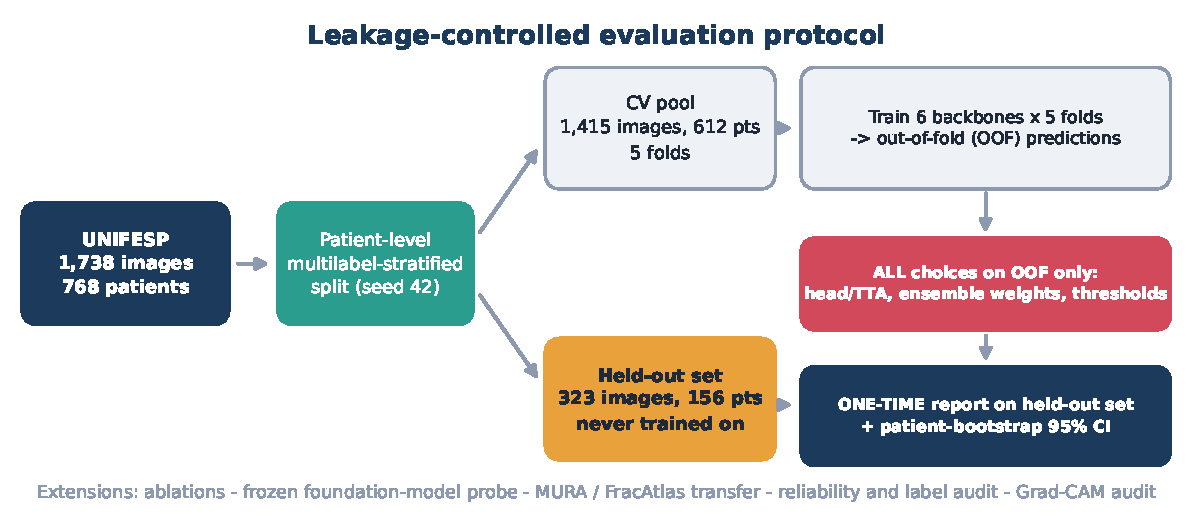
\includegraphics[width=\textwidth]{fig1_protocol.pdf}\caption{Leakage-controlled evaluation protocol.}\label{fig:protocol}\end{figure}
\begin{figure}[H]\centering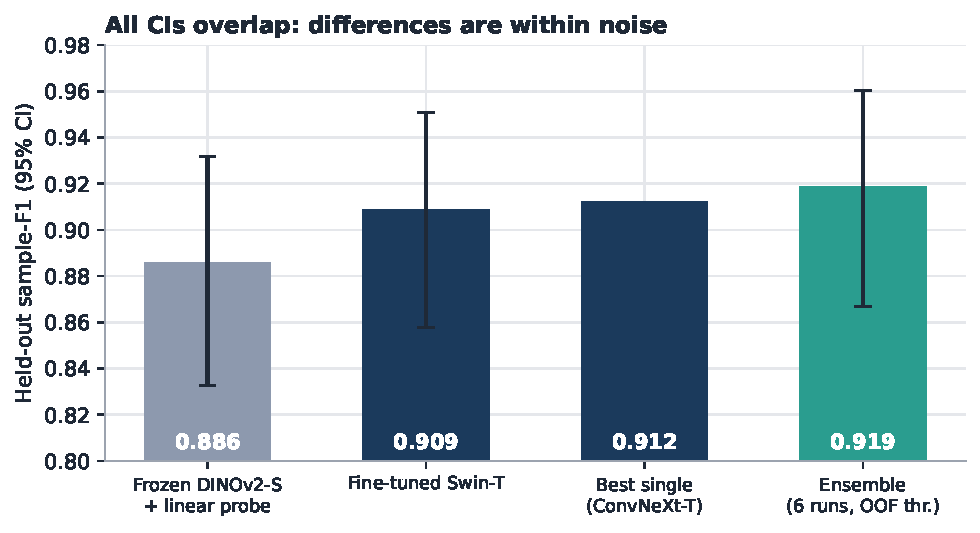
\includegraphics[width=\textwidth]{fig10_heldout_overview.pdf}\caption{Held-out sample-F1 of a frozen-encoder probe, the fine-tuned Swin-T, the best single model and the ensemble; all 95\% CIs overlap.}\label{fig:overview}\end{figure}
\begin{figure}[H]\centering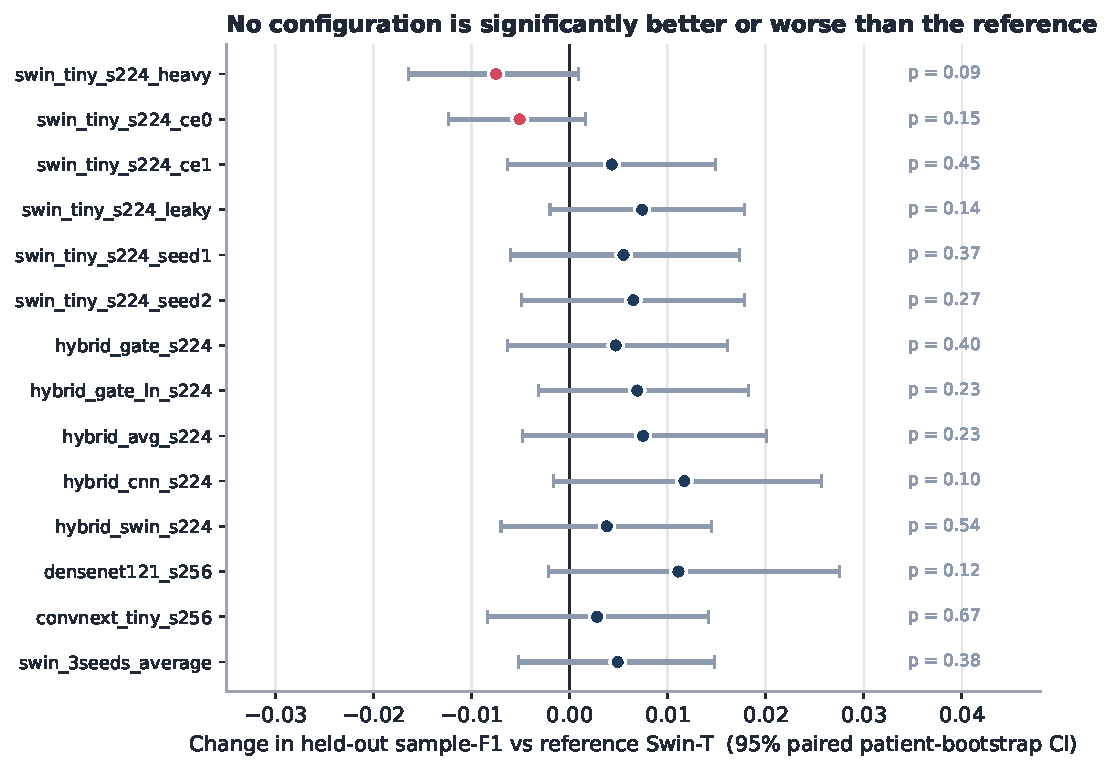
\includegraphics[width=.9\textwidth]{fig2_ablation_forest.pdf}\caption{Ablations: change in held-out sample-F1 versus the reference Swin-T (95\% paired patient-bootstrap CI, p-values on the right).}\label{fig:ablation}\end{figure}
\begin{figure}[H]\centering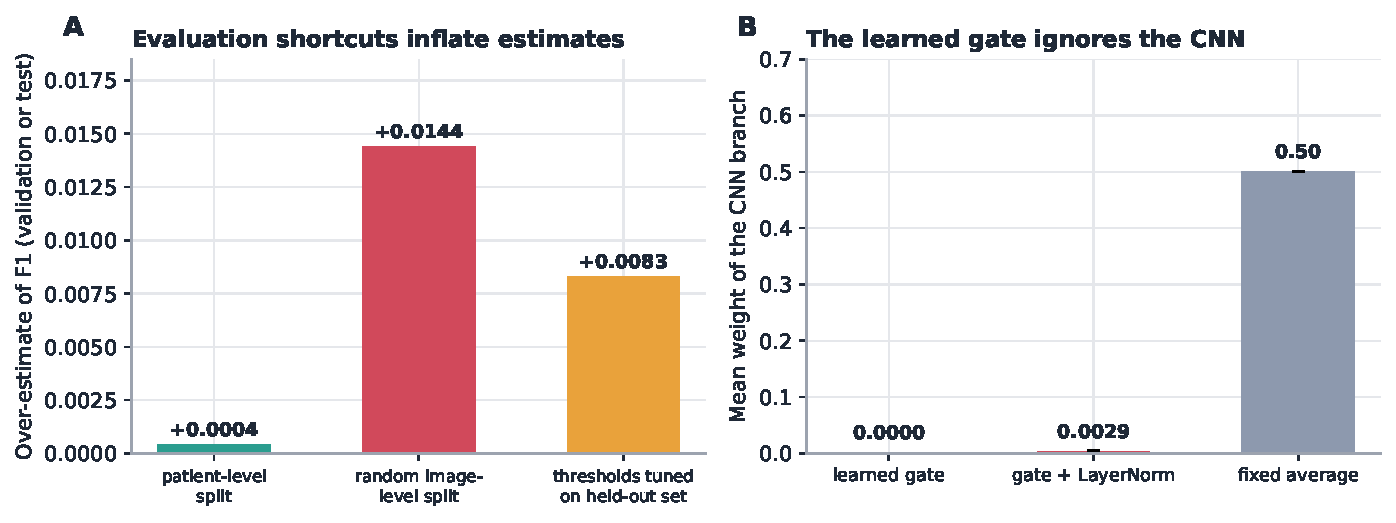
\includegraphics[width=\textwidth]{fig7_leakage_and_gate.pdf}\caption{(A) Over-estimation caused by a random image-level split and by tuning thresholds on the held-out set. (B) Mean CNN-branch weight of the learned gates versus a fixed average.}\label{fig:leakgate}\end{figure}
\begin{figure}[H]\centering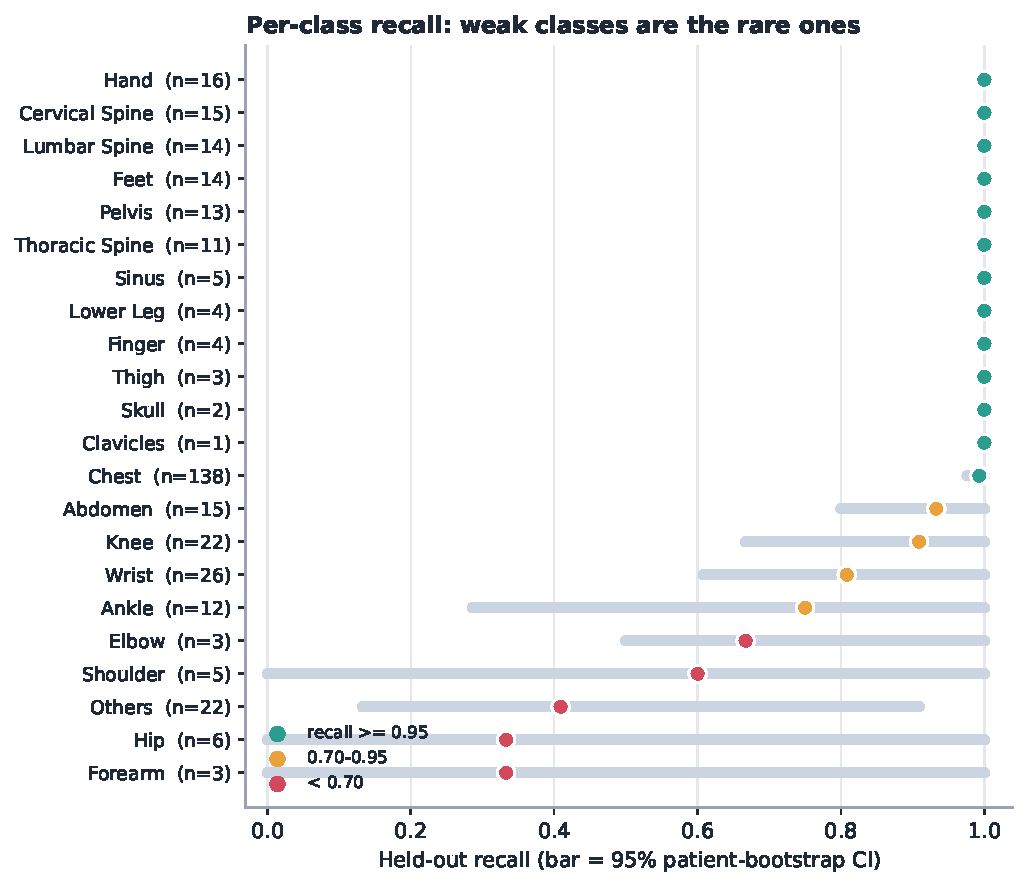
\includegraphics[width=.85\textwidth]{fig3_per_class_recall.pdf}\caption{Per-class held-out recall with patient-bootstrap CIs.}\label{fig:perclass}\end{figure}
\begin{figure}[H]\centering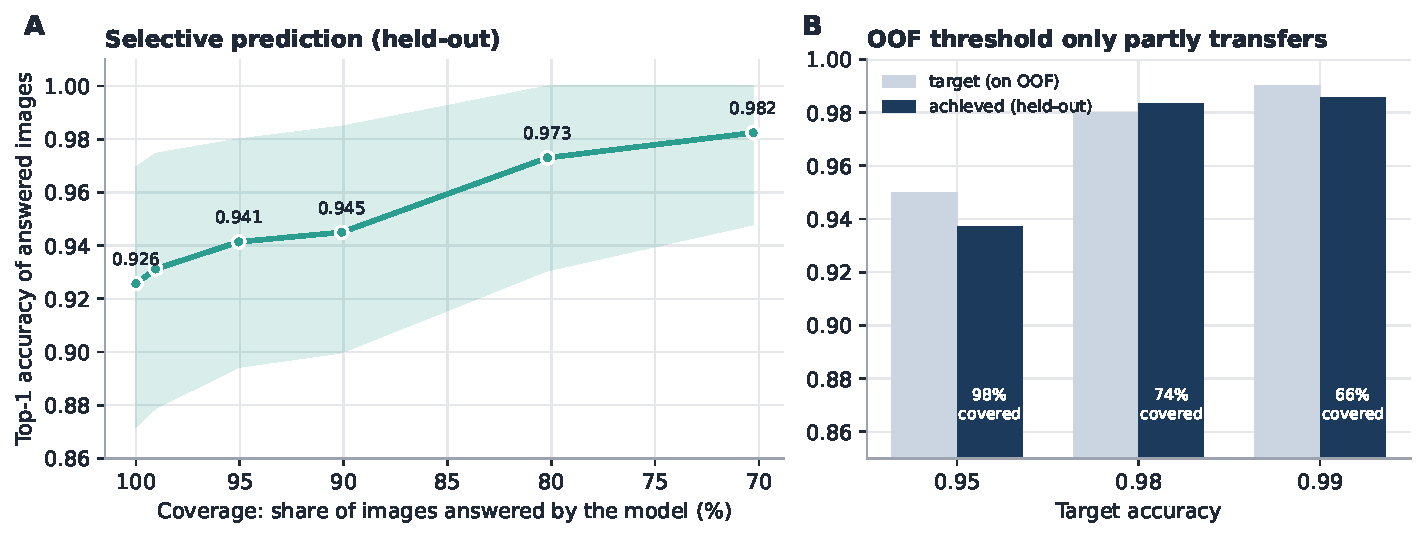
\includegraphics[width=\textwidth]{fig4_reliability.pdf}\caption{(A) Accuracy of answered images versus coverage. (B) OOF-chosen accuracy targets versus achieved held-out accuracy.}\label{fig:reliability}\end{figure}
\begin{figure}[H]\centering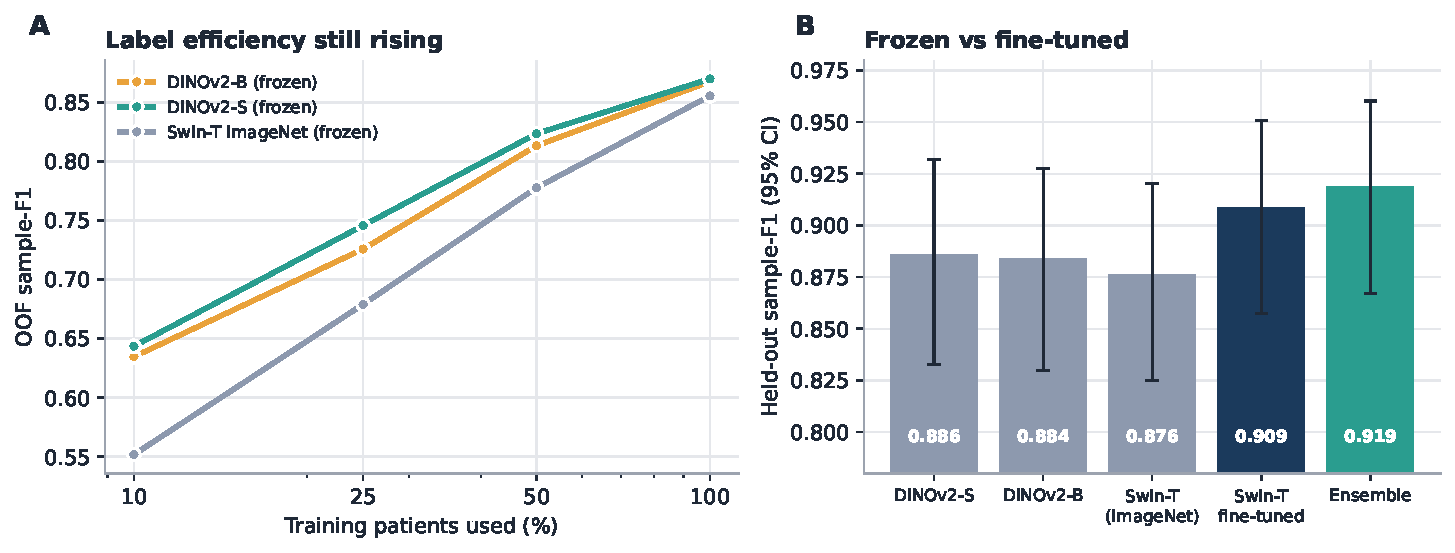
\includegraphics[width=\textwidth]{fig5_foundation_models.pdf}\caption{(A) Label efficiency of frozen encoders. (B) Held-out F1 of frozen probes versus fine-tuned models.}\label{fig:fm}\end{figure}
\begin{figure}[H]\centering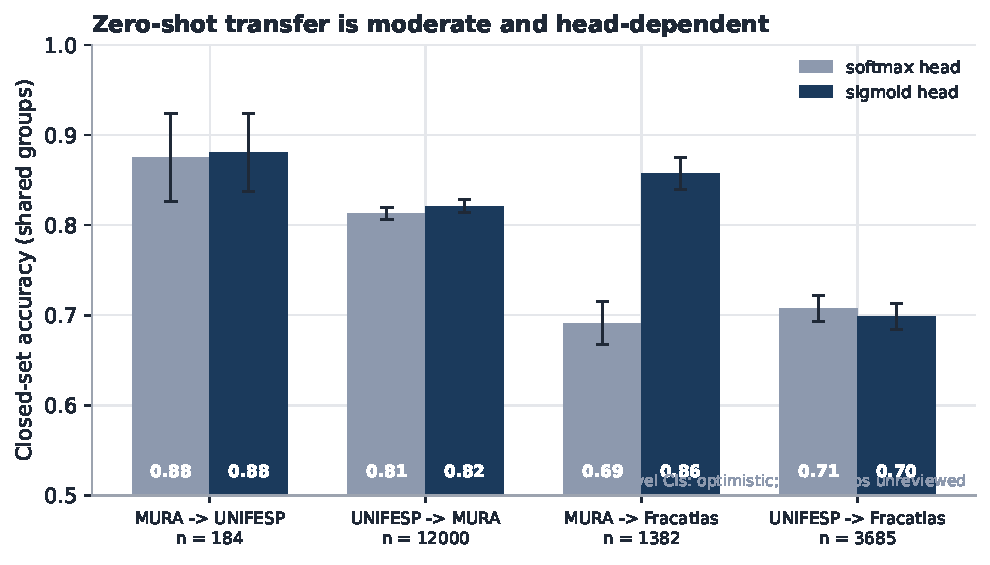
\includegraphics[width=.9\textwidth]{fig6_transfer.pdf}\caption{Zero-shot transfer through the class map (image-level CIs; optimistic).}\label{fig:transfer}\end{figure}
\begin{figure}[H]\centering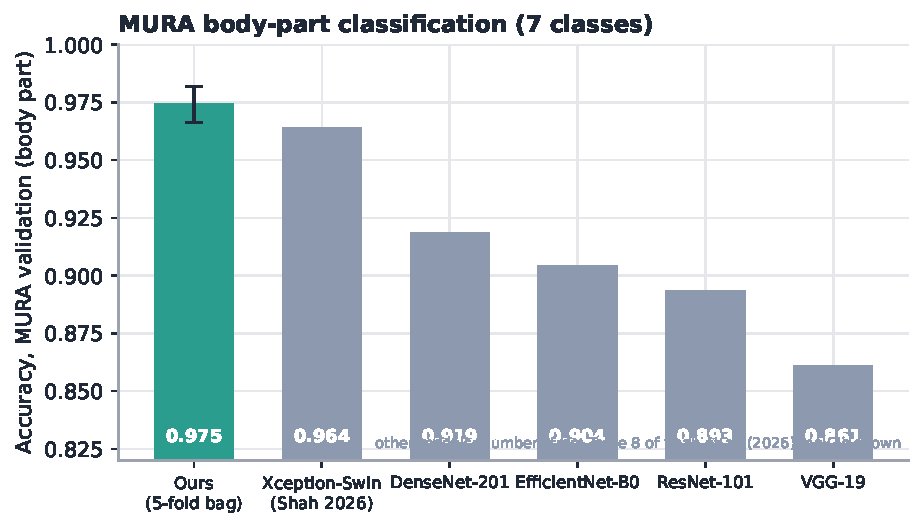
\includegraphics[width=.8\textwidth]{fig9_mura.pdf}\caption{MURA body-part accuracy (7 classes) compared with numbers reported by Shah et al.}\label{fig:mura}\end{figure}
\begin{figure}[H]\centering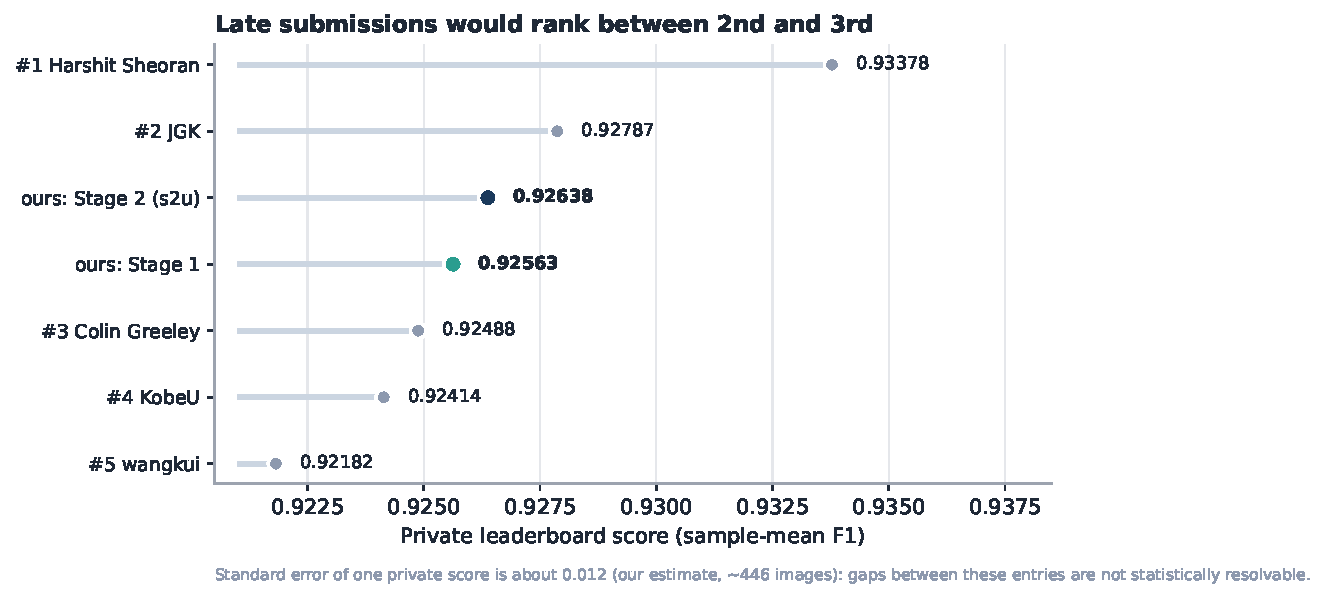
\includegraphics[width=.9\textwidth]{fig8_kaggle.pdf}\caption{Private leaderboard context; ours are late submissions.}\label{fig:kaggle}\end{figure}
\begin{figure}[H]\centering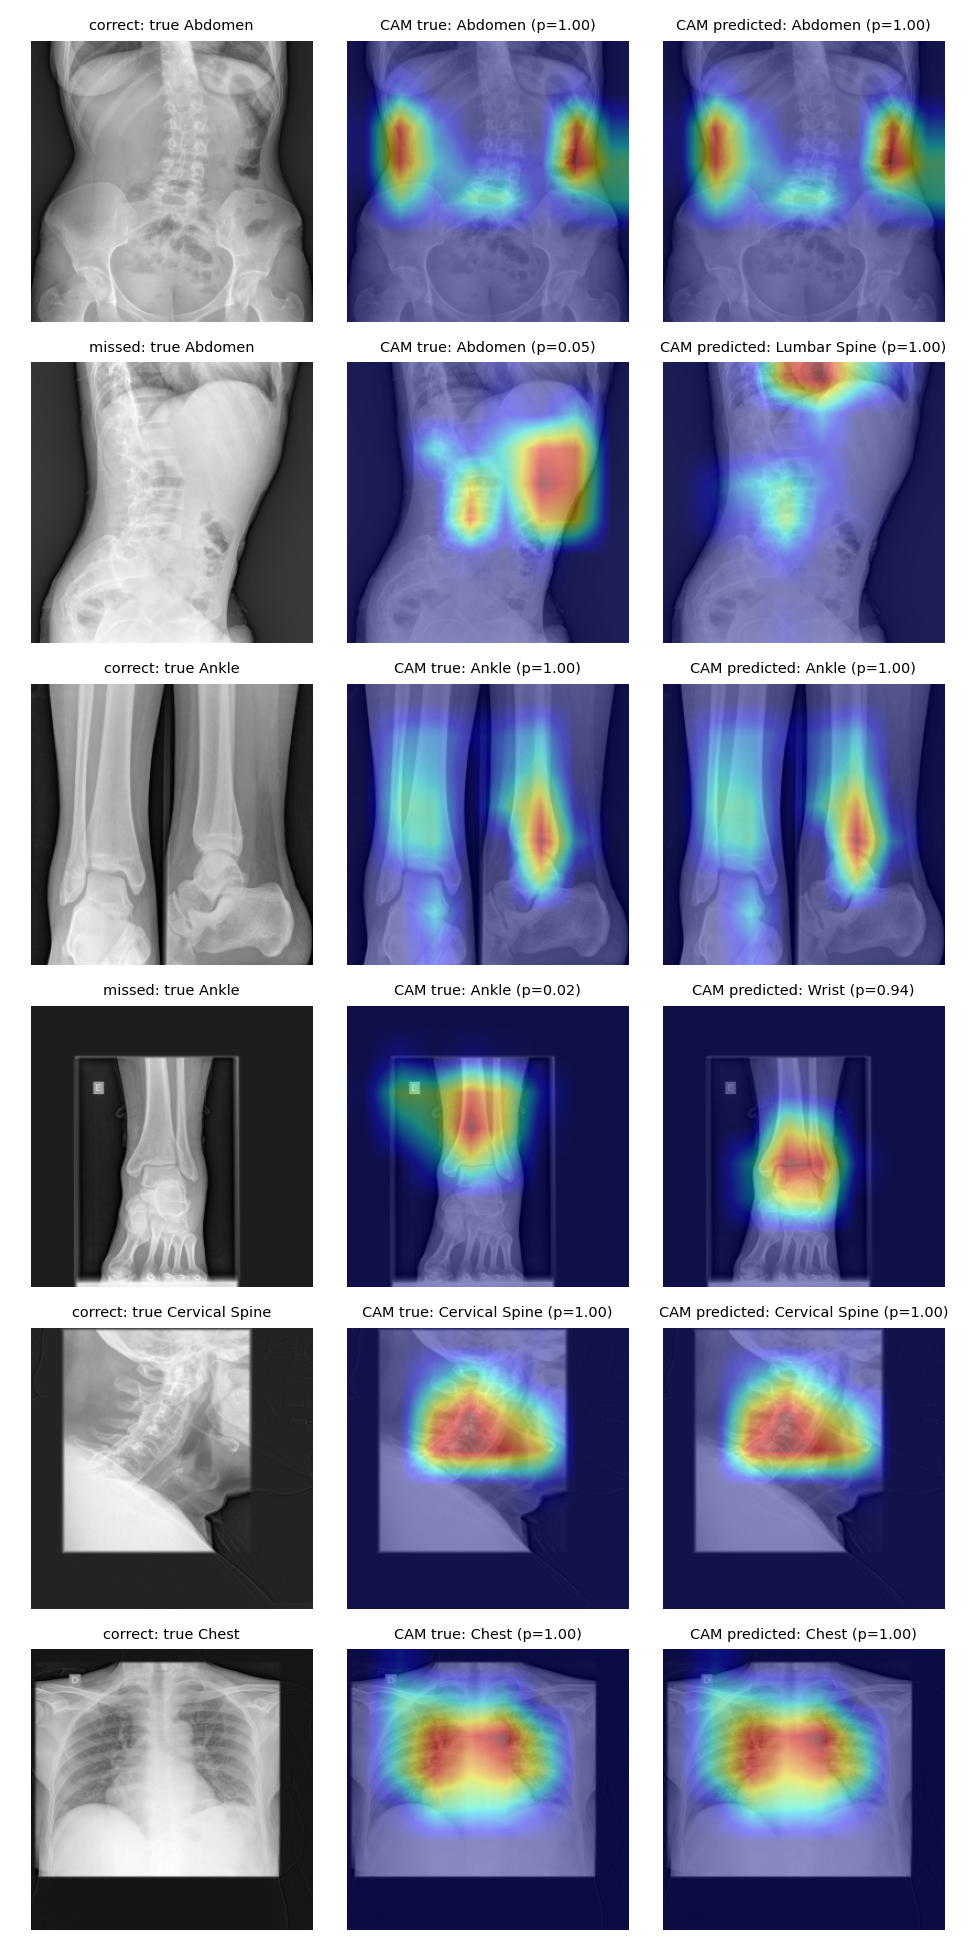
\includegraphics[width=.32\textwidth]{gradcam_gallery_1.png}\hfill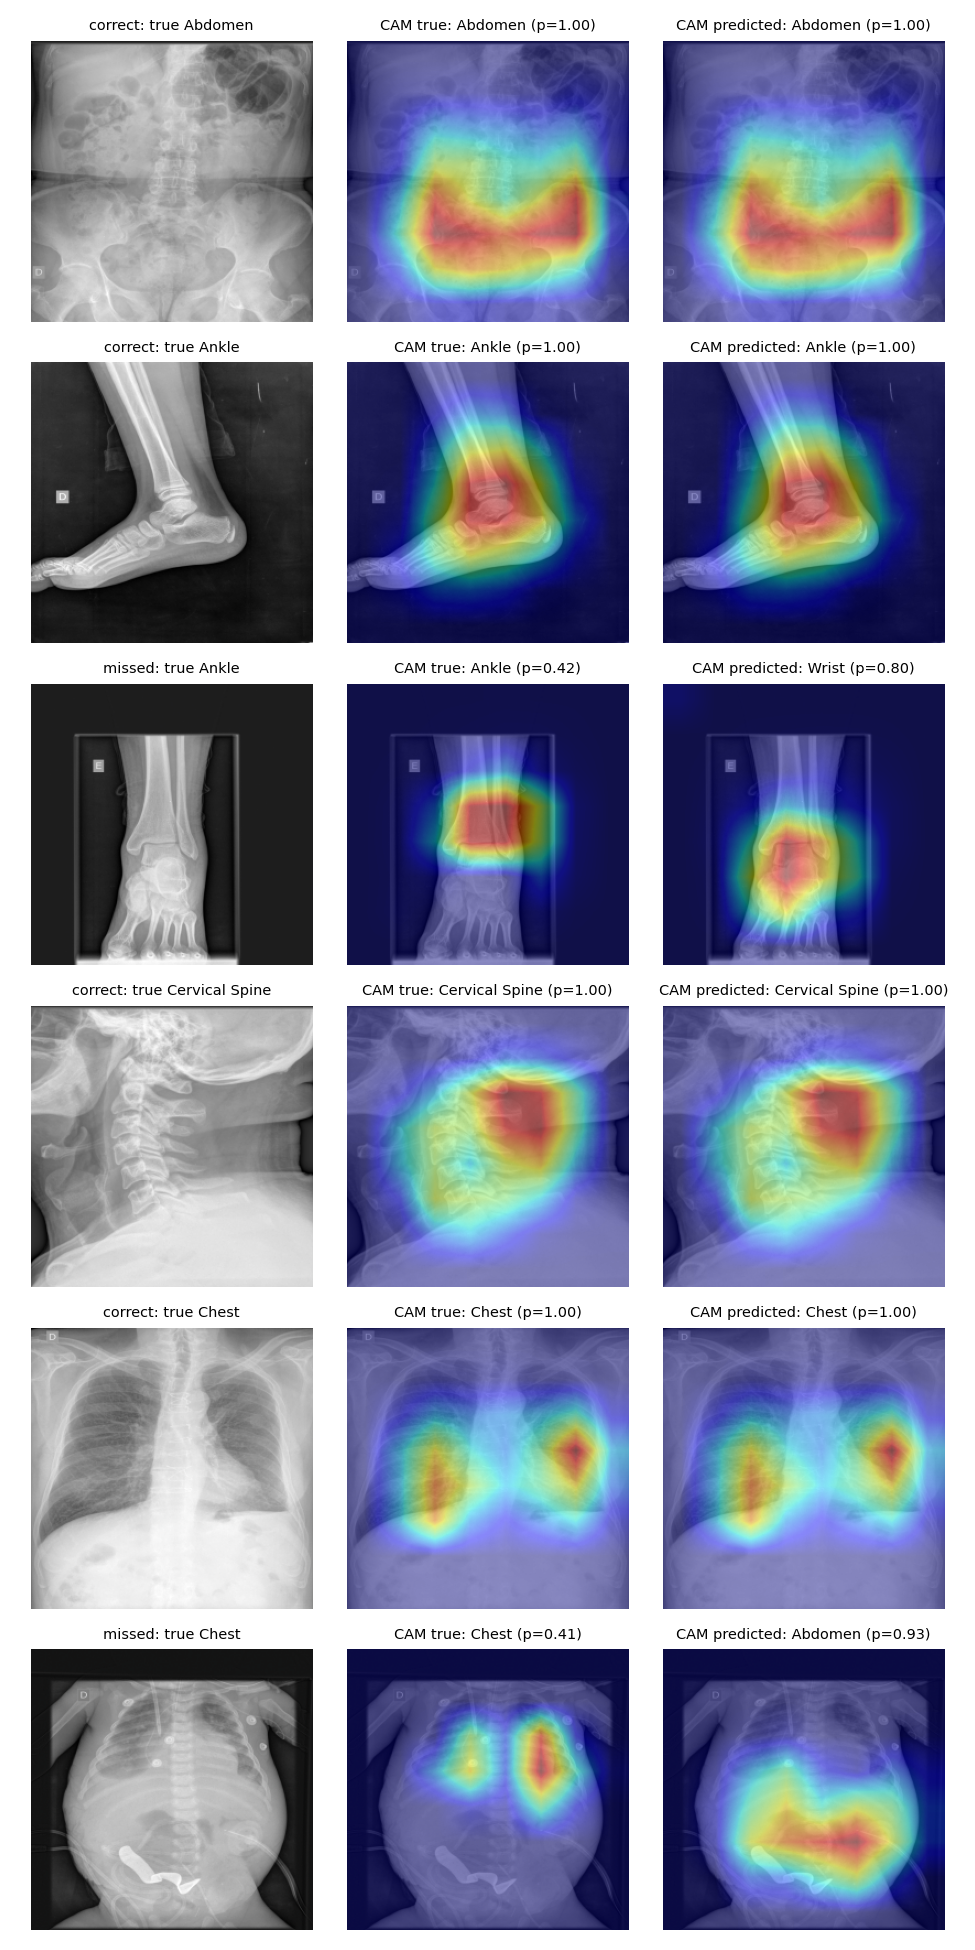
\includegraphics[width=.32\textwidth]{gradcam_gallery_2.png}\hfill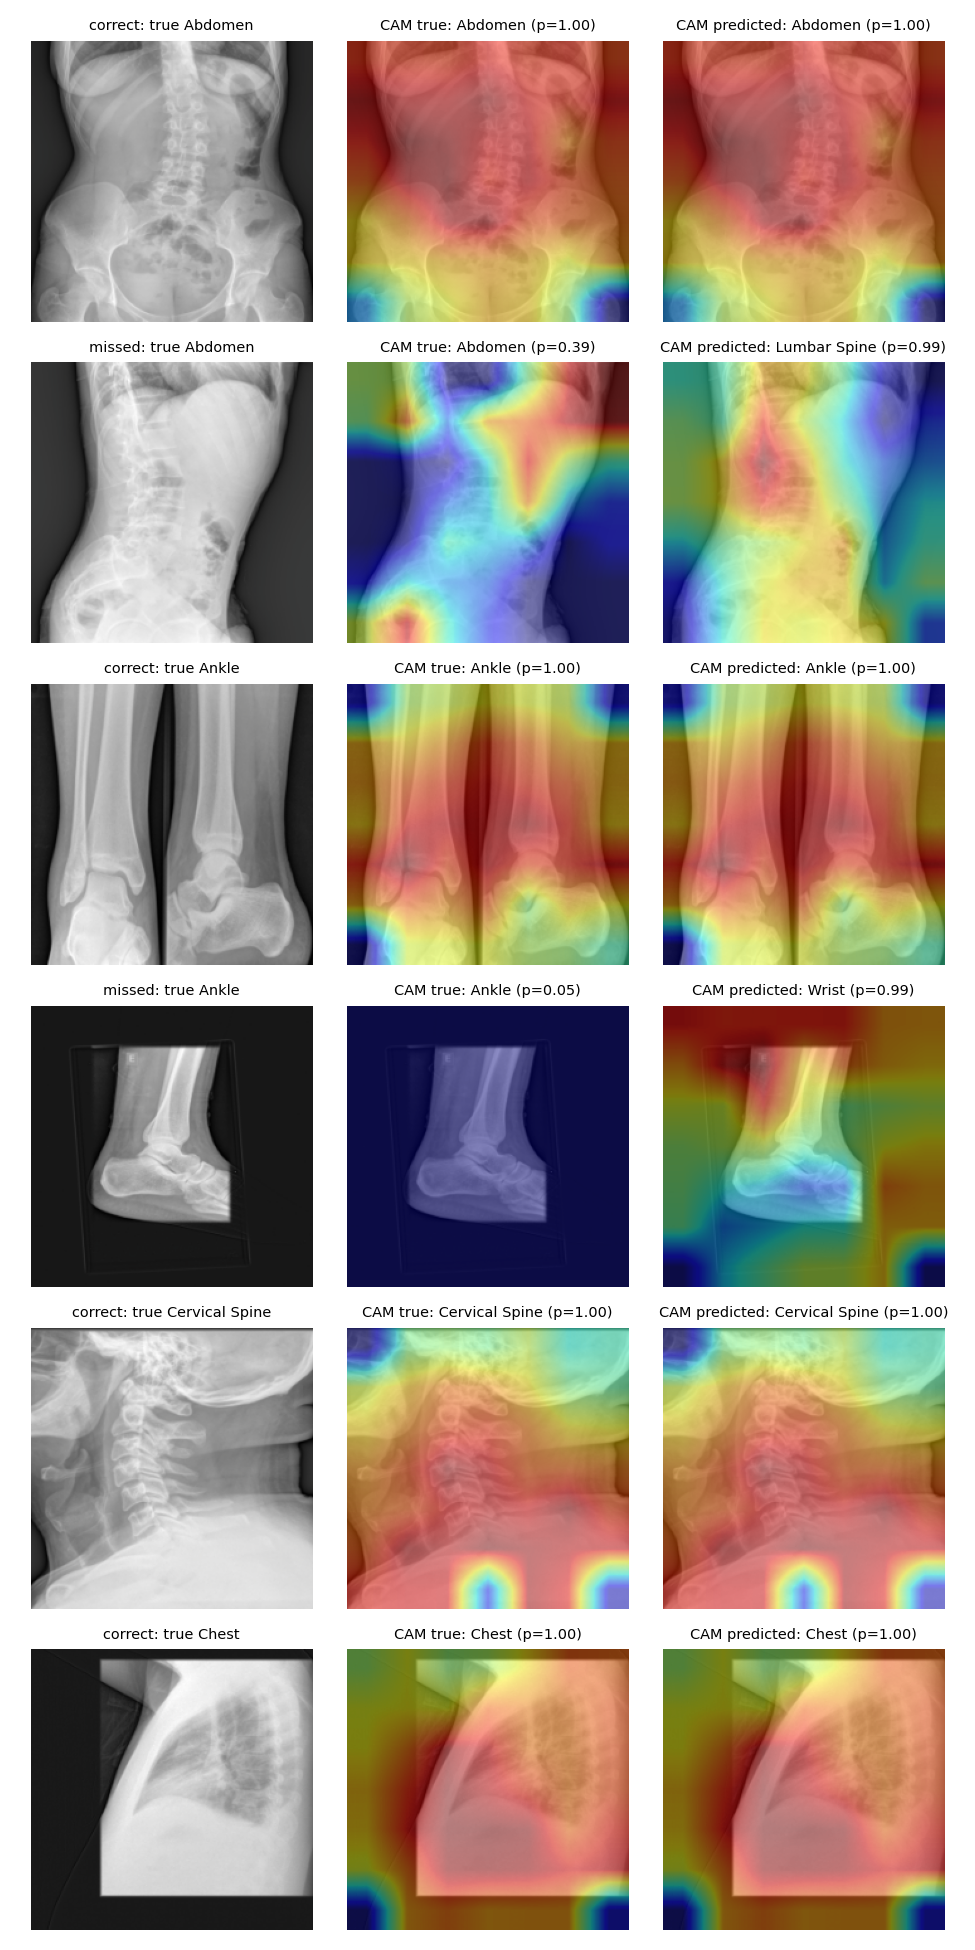
\includegraphics[width=.32\textwidth]{gradcam_gallery_3.png}\caption{Grad-CAM galleries (ConvNeXt-T, ResNet50, Swin-T in notebook order): per class one correct and one missed held-out image; map for the true class and for the predicted class.}\label{fig:gradcam}\end{figure}
\end{document}
